% Documento principal do latex para uso no TCC da Univás.

\documentclass[a4paper, 12pt, chapter=TITLE, oneside, english, brazil]{abntex2}

\usepackage{styles/CodeStyle}      %Formatação de códigos e listagens
\usepackage{styles/EventFlowStyle} %Estilo para o quadro de fluxo de eventos
\usepackage{styles/NuapaStyle}     %Estilo exigido pela Univás
\usepackage{url}
\usepackage{inputenc}
\usepackage{verbatim}
%Início do documento
\begin{document}



\pretextual %Início dos Elementos Pré-Textuais


\makeatletter
\renewcommand{\imprimircapa}{%
\begin{capa}%
\begin{center}%
  %{\ABNTEXchapterfont\large\bfseries\MakeUppercase\imprimirinstituicao}\\
  {\MakeUppercase\imprimirinstituicao}\\
  %{\ABNTEXchapterfont\large\MakeUppercase\imprimirautor}\\
  {\MakeUppercase\imprimirautor}\\
  \vspace*{\fill}%
  \vspace*{\fill}%
  \vspace*{\fill}%
  %{\ABNTEXchapterfont\bfseries\Large\MakeUppercase\imprimirtitulo}\\
  {\MakeUppercase\imprimirtitulo}\\
  \vspace*{\fill}%
  {\color{white}%
\abntex@ifnotempty{\imprimirpreambulo}{%
  %\hspace{.45\textwidth
  \hspace{.45\textwidth}
  \begin{minipage}{.5\textwidth}
    \SingleSpacing
    \imprimirpreambulo
  \vspace{.1\textwidth}\\%
  {\imprimirorientadorRotulo:~\imprimirorientador}
  \abntex@ifnotempty{\imprimircoorientador}{%
    \hspace{.45\textwidth}
    %{\large\imprimircoorientadorRotulo~\imprimircoorientador}%
    {\imprimircoorientadorRotulo~\imprimircoorientador}%
  }%
  \end{minipage}%
}%
\color{black}}%
  \vspace*{\fill}\\%
  %{\large\bfseries\MakeUppercase\imprimirlocal}\\
  %{\large\bfseries\MakeUppercase\imprimirdata}
    {\MakeUppercase\imprimirlocal}\\
    {\MakeUppercase\imprimirdata}
\end{center}
\end{capa}
}
\makeatother

\imprimircapa

% folha de rosto 
%\folhaderostoname{Folha de rosto}
%http://code.google.com/p/abntex2/wiki/ComoCustomizar

\makeatletter
\renewcommand{\folhaderostocontent}{
\begin{center}%
  {\MakeUppercase\imprimirinstituicao}\\%tirei o \Large
  {\MakeUppercase\imprimirautor}\\
  \vspace*{\fill}%
  \vspace*{\fill}%
  \vspace*{\fill}%
  {\MakeUppercase\imprimirtitulo}\\
  \vspace*{\fill}%
\abntex@ifnotempty{\imprimirpreambulo}{%
  \hspace{.45\textwidth}
  \begin{minipage}{.5\textwidth}
    \SingleSpacing
    \imprimirpreambulo
  \vspace{.1\textwidth}\\%
  {\imprimirorientadorRotulo:~\imprimirorientador}
  \abntex@ifnotempty{\imprimircoorientador}{%
    \hspace{.45\textwidth}
    {\imprimircoorientadorRotulo~:\imprimircoorientador}%
  }%
  \end{minipage}%
}%
  \vspace*{\fill}\\%
  %{\ABNTEXchapterfont\large\bfseries\MakeUppercase\imprimirinstituicao}
  %{\large\bfseries\MakeUppercase\imprimirlocal}\\
  %{\large\bfseries\MakeUppercase\imprimirdata}
  {\MakeUppercase\imprimirlocal}\\
  {\MakeUppercase\imprimirdata}
\end{center}
}%end of folhaderostocontent
\makeatother

\imprimirfolhaderosto*{}
\begin{fichacatalografica}
\begin{normalsize}
  \vspace*{\fill}
  % Posição vertical
%  \hrule
  % Linha horizontal
  \begin{center}
  \fbox{
    % Minipage Centralizado
    \begin{minipage}[c]{12.5cm} % Largura
      \vspace{0.7cm}%
      \hspace{0.8cm} \imprimirAutorCitacao ~\\%
      
      \hspace{0.8cm} \imprimirtitulo , \imprimirtipotrabalho. Bacharelado em \imprimircurso. \imprimirlocal - Univás,  \imprimirdata. \pageref{LastPage}p. %
      
      
      
      
      
      

      \hspace{0.8cm} 1. \imprimirPalavraChaveUm. 2. \imprimirPalavraChaveDois. 3. \imprimirPalavraChaveTres. ~ \\%
    \end{minipage}
    }
  \end{center}
\end{normalsize}
\end{fichacatalografica}
\newpage

\begin{comment}

%\imprimirAutorUm , \imprimirAutorDois ~--

\hspace{0.8cm} \imprimirtipotrabalho~--~\imprimirinstituicao , Univás, Bacharelado em \imprimircurso. % 
f. : il.~\\%
 \hspace{0.8cm} \pageref{LastPage}p.
\hspace{0.8cm} \imprimirorientadorRotulo: \\% ~\imprimirorientador ~
\end{comment}
\setlength{\ABNTEXsignwidth}{10cm}

\begin{folhadeaprovacao}
  \begin{center}
    {\large\MakeUppercase\imprimirautor}
    %{\ABNTEXchapterfont\large\MakeUppercase\imprimirautor}
    \vspace*{\fill}
    \vspace*{\fill}
    \vspace*{\fill}
    \par
    {%\ABNTEXchapterfont\bfseries\Large\MakeUppercase\imprimirtitulo}
    {\Large\MakeUppercase\imprimirtitulo}
    \vspace*{\fill}
  \end{center}
  Trabalho de conclusão de curso defendido e aprovado em \imprimirDataDaAprovacao ~pela banca examinadora constituída pelos professores:

  ~\newline
  \begin{flushleft}
  \assinatura*{\imprimirorientador \\ \imprimirorientadorRotulo }
  \assinatura*{\imprimirAvaliadorUm \\ \imprimirAvaliadorLabelUm }
  \assinatura*{\imprimirAvaliadorDois \\ \imprimirAvaliadorLabelDois}
  \end{flushleft}
  \vspace*{\fill}
  \vspace*{\fill}
\end{folhadeaprovacao}




\begin{dedicatoria}


\vspace*{\fill}
\vspace*{\fill}
\vspace*{\fill}
\vspace*{\fill}
\vspace*{\fill}
\vspace*{\fill}
De \imprimirAutorUm.
\newline
%início da dedicatória do autor um
\par Dedico primeiramente a Deus este trabalho, por me dar forças em todos os momentos difíceis que passei e saúde para conquistar todos os objetivos.
\par Dedico aos meus pais Ismauro Sousa Novais e Dalila Cangussú Magalhães de Souza e a toda minha família por me ajudar em todos os momentos dessa caminhada.
A todos os amigos e colegas de faculdade e professores que me ajudaram em algum momento na realização desse sonho de completar o ensino superior para o meu crescimento intelectual e profissional.
 \ldots 

\vspace*{\fill}
De \imprimirAutorDois.
\newline
%início da dedicatória do autor dois
\par Dedico primeiramente a DEUS este trabalho por ter me dado saúde e persistência para a realização desse projeto e por esses 4 anos de faculdade.
\par Dedico aos meus pais Nilsa Franco e Valter de Oliveira e a todos os meus familiares por terem me ajudado e auxiliado em todos os momentos dessa caminhada, para assim conseguir realizar esse sonho de concluir a minha graduação.
\par \ldots

\end{dedicatoria}



\begin{agradecimentos}

De \imprimirAutorUm
\newline
%início do agradecimento do autor um
\par Agradeço primeiramente a Deus por me ajudar em todos os momentos dessa caminhada para realização deste trabalho, me dando muita saúde e paciência.
Aos meus pais Ismauro Sousa Novais e Dalila Cangussú Magalhães de Souza por me apoiarem tanto, dando amor e carinho e me ajudando financeiramente nas dificuldades para pagar as mensalidades da faculdade.
\par Agradeço a Laís Vidal de Oliveira por me ajudar nesse trabalho e tantos outros no decorrer do curso na faculdade e segurar a barra quando precisei me ausentar e pela sua paciência.
E ao professor Ednardo David Segura  por sempre nos motivar a enfrentar novos desafios e por transmitir boa parte do seu conhecimento e sua paixão em sempre ensinar aos seus alunos e dar o seu apoio, que foi fundamental.
\par Aos meus colegas de faculdade por ajudarem nos trabalhos e pelo apoio, motivando e sempre ajudando quando necessário.
E ao meu grande amigo Nícolas Alberto de Paiva e Fernandes em todos esses anos de amizade, me ajudando a melhorar minha capacidade profissional, intelectual e pessoal, além de me ajudar quando podia durante a realização deste trabalho dando, seus palpites.
\par Agradeço por todas as pessoas que passaram nessa minha caminhada que adicionaram algo e ajudaram na conclusão de mais uma etapa em minha vida.
  \ldots \\


\vspace*{\fill}
De \imprimirAutorDois.
\newline
%início do agradecimento do autor dois
\par Agradeço primeiramente a DEUS por seu cuidado comigo, por me ajudar nessa caminhada com paciência e me dando saúde, para a realização deste trabalho.
\par Agradeço imensamente aos meus pais Nilsa Franco e Valter de Oliveira, por todo apoio, dedicação e ajuda financeira no decorrer desses 4 anos de faculdade, por sempre acreditarem no meu potencial, mesmo quando eu nem mesma acreditava, por sempre me aconselharem, mostrando o melhor caminho a seguir e me ajudando naquilo que estava ao alcance de vocês, os meus mais sinceros agradecimentos, pois vocês são as peças fundamentais na minha vida, obrigada por terem sonhado esse sonho comigo, vocês são meus exemplos e meu orgulho e  sem vocês nada disso seria possível. Meu muito obrigado!
\par Agradeço ao meu companheiro Isnack Souza Novais por toda paciência e ajuda para o desenvolvimento desse trabalho e tantos outros no decorrer da faculdade, por ter sido compreensivo quando eu precisei me ausentar, o meu muito obrigada.
\par Ao meu professor e orientador Ednardo David Segura por toda sua disponibilidade em estar sempre nos ajudando e motivando, mostrando que somos capazes de alcançar todos os nossos objetivos e nunca desistir, seu apoio nesse projeto foi de extrema importância, pois sem sua ajuda nada disso seria possível, muito obrigada.
\par Aos meus mestres professores que me acompanharam e compartilharam seus conhecimentos comigo, sempre me auxiliando e mostrando que eu era capaz de ser sempre melhor, obrigada por esses 4 anos. 
\par Agradeço ao meu amigo Nícolas Alberto por toda sua ajuda, seus palpites e sua disponibilidade em estar ajudando neste trabalho, e em outros trabalhos da faculdade, muito obrigada meu amigo.
\par Agradeço aos meus Avós, tios, primos e amigos por todo apoio, por acreditarem em mim e por toda a ajuda que eu recebi no desenvolvimento deste trabalho. E aos meus amigos e colegas de faculdade por esses 4 anos de convivência, por sempre me motivarem e estarem comigo no decorrer desses anos.

\ldots

\end{agradecimentos}







\begin{comment}
‘‘
\end{comment}


\begin{epigrafe}
\vspace*{\fill}
\begin{flushright}
\textit{" Testes podem mostrar a presença de erros, \\
mas não sua ausência. " \\
(E.W.Dijkstra)}
\end{flushright}
\end{epigrafe}









% --- resumo em português ---

\begin{OnehalfSpacing} 

\noindent \imprimirAutorCitacaoMaiuscula. {\bfseries\imprimirtitulo}. {\imprimirdata}.  Monografia -- Curso de {\MakeUppercase\imprimircurso}, {\imprimirinstituicao}, {\imprimirlocal}, {\imprimirdata}.

\vspace{\onelineskip}
\vspace{\onelineskip}
\vspace{\onelineskip}
\vspace{\onelineskip}

\begin{resumo}
~\\
%início do texto do resumo
\begin{comment}


\noindent Este trabalho apresenta \ldots
 \end{comment}
 
 
 \par Atualmente há uma grande demanda de desenvolvimento de \textit{software}, e com isso o usuário final exige um sistema com o menor número de \textit{bugs} possíveis. Neste contexto, foi feita a demonstração e utilização dos testes automatizados de \textit{software}, por meio da prática de desenvolvimento TDD, que mostra como os testes ajudam a entregar um sistema de qualidade e com uma taxa mínima de erros. Durante a pesquisa foi desenvolvida uma folha de pagamento \textit{web} e através dela foram realizados todos os testes propostos para esta aplicação. Foi utilizada em conjunto com os testes automatizados, a integração contínua, que visa a cada nova melhoria no sistema verificar se os testes irão passar novamente ou se irão quebrar a \textit{build}, e o relatório de cobertura, que auxilia o desenvolvedor a visualizar qual é o índice de cobertura do código e qual parte do sistema necessita de mais testes. A utilização dessas ferramentas só agregam e ajudam no processo de desenvolvimento dos \textit{softwares}, pois possui \textit{fast feedback} (retorno rápido) para o desenvolvedor, que facilita na detecção e solução de problemas e visa produzir um sistema com o menor índice de erros. Este trabalho foi desenvolvido por meio de pesquisa aplicada, visando otimizar o resultado final, com o objetivo de resolver problemas específicos identificados durante todo o desenvolvimento dos testes.
 
 
 
 \begin{comment}
 

 Este trabalho enquadra-se no tipo de pesquisa aplicada, pois foi desenvolvido um sistema com o objetivo de resolver problemas específicos. 
 

 
 
 
 
Palavras-chave:
 \end{comment}
%fim do texto do resumo
\vspace{\onelineskip}
\vspace*{\fill}
\noindent \textbf{Palavras-chave}: \imprimirPalavraChaveUm. \imprimirPalavraChaveDois. \imprimirPalavraChaveTres.
\vspace{\onelineskip}
\end{resumo}

\end{OnehalfSpacing}









% --- resumo em inglês ---

\begin{OnehalfSpacing} 

\noindent \imprimirAutorCitacaoMaiuscula. {\bfseries\imprimirtitulo}. {\imprimirdata}.  Monografia -- Curso de {\MakeUppercase\imprimircurso}, {\imprimirinstituicao}, {\imprimirlocal}, {\imprimirdata}.

\vspace{\onelineskip}
\vspace{\onelineskip}
\vspace{\onelineskip}
\vspace{\onelineskip}

\begin{resumo}[\textit{Abstract}]%
\begin{otherlanguage*}{english}%



\par \textit{Nowadays there is a great demand of software development and with this the final user requires a system with the least amount of defects possible. In this context was made a demonstration and usage of automated tests of softwares through the TDD method, which shows how the tests help to deliver a quality system and with a minimal rate of errors. During the research a web payroll was developed and through it all the automated tests proposed by this application
were applied. Used alongside the automated tests was the continuous
integration, which in every new improvement in the system aims to verify if all the tests will pass once more or if they will break the build, and the cover report which assists the developer to visualize the cover rate of the code and which part of the system needs more tests. The use of these tools only add and help in the process of software development because it has fast feedback which facilitates in the detection and solution of problems and aims to produce a system with the lowest error rates. This academic project was developed through applied research aiming to optimize the final result, with the objective to resolve specific problems identified during all the tests development.}

\vspace{\onelineskip}
\vspace*{\fill}
\noindent \textbf{Key words}: \imprimirKeyWordOne. \imprimirKeyWordTwo. \imprimirKeyWordThree.
\end{otherlanguage*}
\vspace{\onelineskip}
\end{resumo}

\end{OnehalfSpacing}



%Lista de Figuras
\pdfbookmark[0]{\listfigurename}{lof}
\listoffigures*
\cleardoublepage

% Lista de Quadros
%\pdfbookmark[0]{\listofquadrosname}{loq}
%\listofquadros*
%\cleardoublepage

%Lista de Tabelas
%\pdfbookmark[0]{\listtablename}{lot}
%\listoftables*
%\cleardoublepage

%Lista de Códigos
\counterwithout{lstlisting}{chapter}
\pdfbookmark[0]{\lstlistingname}{lol}
%http://tex.stackexchange.com/questions/50031/how-to-remove-contents-line-from-table-of-contents
\begin{KeepFromToc}
\lstlistoflistings
\end{KeepFromToc}
\cleardoublepage








%Lista de siglas
%ver http://marc.info/?l=tex-br&m=110566665520790 para colocar em ordem alfabética.

\begin{SingleSpace}
\begin{siglas}
 
\item[BDD] \textit{Behavior Drive Developmen}
\item[CI] \textit{Continuous Integration}
\item[CSS] \textit{Cascading Style Sheet}
\item[HTML] \textit{HyperText Markup Language}
\item[HTTP] \textit{HyperText Transfer Protocol}
\item[INSS] \textit{Instituto Nacional de Seguro Social}
\item[IR] \textit{Imposto de Renda}
\item[I/O] \textit{Input/Output}
\item[JS] \textit{JavaScript}
\item[JSON] \textit{JavaScript Object Notation}
\item[MTPS] \textit{Ministério do Trabalho e Previdência Social}
\item[NPM] \textit{Node Packager Manager}
\item[REST] \textit{Representational State Transfer}
\item[SO] \textit{Sistema Operacional}
\item[TDD] \textit{Test Driven Development}
\item[URL]  \textit{Universal Resource Locator}
\item[XP] \textit{Extreme Programming}
\item[W3C] \textit{World Wide Web Consortium}



\end{siglas}

\end{SingleSpace}

%Sumário
%ver esse link para configuração de fonte: http://tex.stackexchange.com/questions/83377/how-to-change-chapter-font-style-in-the-middle-of-the-table-of-the-contents
\pdfbookmark[0]{\contentsname}{toc}
\begin{SingleSpace} 
\tableofcontents*
\end{SingleSpace}
\cleardoublepage



\textual %Início dos Elementos Textuais

%\chapter*{Introdução}
\begin{flushleft}
	\vspace{1.2em}
	\textbf{\large INTRODUÇÃO}
	\vspace{2.9em}
\end{flushleft}
%\thispagestyle{empty}

\addcontentsline{toc}{chapter}{INTRODUÇÃO}
\stepcounter{chapter} %incrementa o número do capítulo

\par Com o constante avanço do desenvolvimento de \textit{software}, cada vez mais se encontram sistemas complexos e de alta criticidade espalhados pelo mundo. Quanto mais crítico e complexo é o sistema,  maior é a necessidade de que o sistema seja executado com precisão, minimizando os erros.

\par As empresas procuram aprimorar e aperfeiçoar o desenvolvimento de \textit{softwares}, fazendo com que os usuários tenham mais confiança e segurança na utilização dos sistemas.

\par Devido à complexidade e inúmeras dificuldades relacionadas ao processo de desenvolvimento dos \textit{softwares}, que envolvem as questões humanas, burocráticas e políticas. As empresas têm um grande desafio para controlar a qualidade destes \textit{softwares} para os usuários finais. Os sistemas precisam fazer corretamente o que foi solicitado pelo cliente, de forma segura, eficiente e de fácil manutenção e evolução \cite{ime},s.p.

\par Para auxiliar as empresas de desenvolvimento de \textit{software}, surgiram processos de testes automatizados. Segundo \citeonline{qualister}, "o propósito da automação de testes pode ser resumidamente descrito como a aplicação de estratégias e ferramentas, tendo em vista a redução do envolvimento humano em atividades manuais repetitivas".

\par Há 10 anos foi realizada uma pesquisa pela Forrester Research Inc em que 9\% das empresas(Estados Unidos e Reino Unido) utilizavam testes em seus processos, a fim de diminuir correções e retrabalhos nos \textit{softwares}, aumentando a satisfação do usuário final com um sistema mais preciso possível \cite{qualister}.

\par Diariamente, algumas tarefas são repetidas diversas vezes, ocasionando um desgaste natural em seus executores. Tarefas repetitivas são, muitas vezes, morosas àqueles que as executam, o que pode gerar falhas e comprometer o procedimento a ser executado. No mundo de desenvolvimento de \textit{softwares} não é diferente. Há tarefas repetitivas e custosas aos que as colocam em execução. Muitas vezes, pessoas erram e podem ocasionar falhas nestes procedimentos. Certos problemas ocasionados podem gerar desconforto para as empresas, como a insatisfação do cliente final com determinados problemas e erros que não foram verificados com cautela.

\par Os testes automatizados surgiram para auxiliar este cenário acima citado. São eles os responsáveis por verificar constantemente o bom funcionamento de uma aplicação, a fim de verificar se há problemas que possam comprometer o sistema. Com isso, um \textit{software} com maior qualidade é disponibilizado ao cliente final, pois os erros comuns são encontrados através desta abordagem. Além do mais, os testes automatizados se tornam eficazes, pois é possível criar cenários complexos e elaborados para testes com o intuito de analisar toda e qualquer probabilidade de erro, o que toma muito tempo hábil de um desenvolvedor caso o mesmo fosse feito manualmente.

\par Os testes podem ser resumidamente descritos como a aplicação de estratégias e ferramentas tendo em vista a redução do envolvimento humano em atividades manuais repetitivas.

\par Para isso, usa-se o teste de \textit{software} para poder testar a aplicação no desenvolvimento, o qual pode incluir uma aplicação \textit{web}, aplicativos para celular, entre outros. Nesse procedimento é possível fazer verificações do funcionamento das aplicações para que se possa evitar erros futuros. Este uso representa ganhos para a empresa, tais como: significativa economia de esforço, aumento da qualidade do sistema, diminuição do custo de manutenção e o aumento da satisfação do cliente, dentre outros.

\par Ao fazer o teste de \textit{software}, entrega-se um produto final de alta qualidade e poucos erros. A empresa tem redução de gastos com a manutenção de aplicações que possam apresentar erros. Por isso, é tão importante falarmos em qualidade, pois está diretamente relacionada com a satisfação. Segundo \citeonline{teste}, "a qualidade não é apenas um diferencial e sim uma meta para se tornar uma empresa mundialmente conhecida."
\par O objetivo geral desse trabalho é demonstrar o funcionamento dos testes automatizados, e para que o objetivo geral fosse alcançado, ele foi dividido em alguns específicos.


\begin{itemize}
    \item Discussão dos testes automatizados;
    \item Demonstração das ferramentas;
    \item Demonstração da utilização dos testes automatizados;
    \item Integração contínua.
\end{itemize}

\par Serão descritas técnicas, tipos de testes e análise de ferramentas, objetivando a análise de processo de testes de \textit{software} automatizado como um processo de desenvolvimento.

\par O trabalho é composto de quatro capítulos, sendo o atual uma breve introdução sobre o tema proposto e seus objetivos. No segundo capítulo foram descritas as teorias sobre as tecnologias utilizadas para o desenvolvimento do projeto. O terceiro, relatou as metodologias usadas na pesquisa, tais como: tipo de pesquisa, contexto de pesquisa, instrumentos e procedimentos.
No quarto capítulo foi realizada a discussão de resultados ressaltando o que se obteve com a realização do trabalho. Por fim, a conclusão.
\begin{comment}



\chapter{Justificativa}

\end{comment}
\begin{comment}



\chapter{OBJETIVOS}


\par Neste capítulo são apresentados os objetivos do projeto.
 
 
\section {Objetivos Gerais}

\par Demonstrar ferramentas, tecnologias e os tipos de testes automatizados. 
  

\section{Objetivos Específicos}
\par Visando atingir o objetivo geral, alguns objetivos específicos são requeridos, entre eles:
\begin{itemize}
    \item Descrever os tipos de testes automatizados;
    \item Demonstrar ferramentas;
    \item Demonstrar a utilização dos testes automatizados;
    \item Ter Integração contínua.
    
\end{itemize}

\end{comment}
\chapter{QUADRO TEÓRICO}

\par Neste capítulo foram descritos os principais conceitos e características das tecnologias a serem utilizadas para o desenvolvimento do \textit {software} utilizado para demonstrar o uso dos testes automatizados.

\section{Técnicas de Testes}

\par As técnicas de testes são ferramentas importantes para a melhoria do \textit{software} no passo a passo do seu desenvolvimento.
\begin{citacao}

 \par Segundo \citeonline{engenharia}" Atualmente existem muitas maneiras de se testar um \textit {software}. Mesmo assim, existem as técnicas que sempre foram muito utilizadas em sistemas desenvolvidos sobre linguagens estruturadas que ainda hoje têm grande valia para os sistemas orientados a objeto. Apesar de os paradigmas de desenvolvimento serem completamente diferentes, o objetivo principal destas técnicas continua a ser o mesmo: encontrar falhas no \textit {software}".
 
\end{citacao}

\par As técnicas de testes são conhecidas como:  Teste Estrutural (caixa branca) e Teste Funcional (caixa preta), os quais serão melhor discutidos a seguir.

 \textbf{Teste Estrutural} é uma técnica também chamada de caixa-branca, que tem por objetivo avaliar o comportamento interno do componente de \textit{software}. Pode-se construir códigos para efetuar a ligação de bibliotecas e componentes \cite{tecnicas}.
 
 \par Nesse tipo de técnica o analista tem total acesso à estrutura interna do \textit{software} a ser analisado e, portanto, os testes são projetados com maior precisão e eficiência.
 
 \par Esse tipo de procedimento é desenvolvido analisando-se o código fonte e elaborando-se casos de teste que cubram todas as possibilidades do componente de \textit software. Dessa maneira, todas as variações originadas por estruturas de condições são testadas. Um exemplo prático desta técnica é o uso da ferramenta JUnit para desenvolvimento de classes de teste (\textit{ test cases}) para verificar classes ou métodos desenvolvidos em Java\cite{engenharia}.

\par Segundo \citeonline{branca}, É um método de projeto de testes que usa a estrutura de controle do projeto procedimental para derivar casos de teste.

 \textbf{Teste Funcional} é uma técnica também chamada de caixa-preta, no qual o componente de \textit{software} a ser testado é abordado como se estivesse dentro de uma caixa preta, cujo conteúdo é desconhecido e na qual só é possível visualizar o lado externo, ou seja, os dados de entrada fornecidos e as respostas produzidas como saída. Portanto, não se leva em consideração o comportamento interno do mesmo.
 
 \par Esse tipo de teste revela a forma como o usuário vê o sistema, pois o interesse dele é servir-se do software sem considerar os detalhes de sua construção. É particularmente útil para revelar problemas, como :
 
 \begin{itemize}
     \item funções incorretas ou omitidas;
     \item erros de interface;
     \item erros de comportamento ou desempenho;
     \item erros de iniciação e término.
 \end{itemize}

 
\par Um exemplo dessa aplicação é verificar a consistência de dados de interface, com isso, o analista implementa entradas erradas de dados e observa qual vai ser o comportamento do \textit{software} \cite{qualidade}.



\section{Fases de Testes}

\par Os testes estiveram presentes em todo o processo de desenvolvimento de \textit{software}, ajudando a reduzir os erros do sistema. E foram divididos nas seguintes fases:

 \textbf{Teste de Unidade}: também conhecido como testes unitários, tem por objetivo testar as menores unidades de software desenvolvidas e encontrar falhas de funcionamento dentro dessa pequena fase testada, independentemente do todo. Além de dar um \textit{fast feedback} \footnote{resposta rápida.} para o desenvolvimento \cite{unidade}.
    
\textbf{Testes de Integração}: as unidades do sistema foram testadas de forma combinada e o objetivo é detectar falhas na interação entre as unidades integradas. Não fazem parte dessa fase os testes de integração com outros sistemas. Esses testes são realizados depois do de unidade e antes do funcional. Ex: Na integração do cadastro de clientes com a função que valida CPF; as duas unidades já foram testadas individualmente na fase de testes de unidade, neste momento é realizada a interação entre elas e feita a validação \cite{integracao}. 
    
\textbf{Teste de Funcional}: o objetivo foi testar o sistema do ponto de vista do usuário final, assim, buscando possíveis falhas; o teste ocorreu dentro de condições similares de ambiente, interfaces e sistêmicas e massas de dados, as quais o usuário executa no seu dia-a-dia.

  \begin{comment}      
\textbf{ Teste de Aceitação}: o objetivo final foi verificar se o sistema desenvolvido está de acordo com o que foi solicitado. É escolhido um grupo restrito de usuários finais para simularem as operações de rotina do sistema.
  

 \textbf{ Teste de Regressão}: não corresponde a um nível de teste, mas é uma estratégia importante para a redução de "efeitos colaterais". Consiste em aplicar, a cada nova versão do software ou a cada ciclo, todos os procedimentos anteriormente aplicados nos mesmos. Para ter o aumento da produtividade e a viabilidade dos testes, é necessário o uso de ferramentas de automação, em uma nova versão ou ciclo, e verificar se foram reexecutados com agilidade e precisão.
\end{comment}    

\section{Test Driven Development - TDD}

\par É uma prática de desenvolvimento de \textit{software} derivado da metodologia \textit{Extreme Programming}, na qual a sua prática consiste em criar os testes primeiramente antes da implementação do código fonte. São feitos os seguintes passos no TDD: primeiramente cria-se um teste e execute-o logo em seguida, após esse teste falhar é feita a implementação do código fonte.

\par Os testes são executados novamente e deverão passar, deste modo, após os testes passarem é necessário verificar a necessidade de melhorar o código. Caso haja alteração no código, os testes serão executados novamente e caso os testes não passem, é feita a correção do erro para os testes passarem novamente. Entre um dos maiores benefícios do TDD é o \textit{feedback} (retorno rápido) para o programador, pois isso é feito de maneira rápida e as falhas são identificadas mais rapidamente \cite{tdd}.

\par O simples ato de inverter a ordem, no caso de realizar os testes antes de codificar, traz diversos benefícios para um projeto.
As baterias de testes tendem a serem maiores  e assim garantindo maior qualidade no código produzido \cite{tdd2}.


\section{Integração Contínua}

\par É um termo originado na metodologia ágil XP\footnote{Extreme Programming}, sua função é simples: o desenvolvedor integra o código que foi alterado e/ou desenvolvido ao projeto principal na mesma frequência com que as funcionalidades são desenvolvidas. Utilizando a integração contínua é possível verificar se as novas alterações ou funcionalidades que foram criadas não causam defeitos no projeto já existente \cite{integracao}.

\newpage
\par Dessa forma os erros de integração podem ser detectados mais rapidamente. Muitas equipes perceberam que essa abordagem leva a uma redução significativa nos problemas de integração \cite{integracao} . 
\begin{citacao}

\par Segundo \citeonline{integracaoContinua}: "Integração Contínua é uma pratica de desenvolvimento de \textit{software} no qual os membros de um time integram seu trabalho frequentemente, geralmente cada pessoa integra pelo menos diariamente – podendo haver múltiplas integrações por dia. Cada integração é verificada por um \textit{build} automatizado (incluindo testes) para detectar erros de integração o mais rápido possível."
\end{citacao}

\par A ferramenta que será utilizada para fazer a integração contínua é o \textit{TravisCI} que será explicado na secção ferramentas.




\section{Relatório de Cobertura}

\par A cobertura mede o quanto um grupo de testes examina a capacidade de um determinado software. É a medida da abrangência do teste, indicando o nível de confiança atribuído a ele.

\par Essa métrica permite verificar se todas as funcionalidades e/ou unidades do sistema estão sendo testadas corretamente. Em um conjunto de itens a serem testados, a cobertura nos mostra a porção a qual foi realmente testada.

\par O relatório de cobertura indica a integridade dos testes, sem tratar da efetividade dos mesmos, podendo ser usado como critério de parada dos testes.

\par Deste modo, a cobertura dos testes é mostrada em porcentagem. Por exemplo, se o resultado de cobertura de testes é de 100\%, isso indica que foi essa a porcentagem de declarações do programa as quais foram analisadas, mas não necessariamente que o sistema como um todo foi realmente testado \cite{relatorio}.

 \subsection{Cobertura de testes baseada em código.}

 \par A medida da cobertura de teste baseada em código é efetuada a partir da quantidade de código executado durante o período de testes em comparação à quantidade total de código pendente de execução.

\par A cobertura pode ser baseada em fluxos de controle ou em fluxos de dados. Nos fluxos de controle são testadas linhas de código, ou seja, se o código foi exercitado pelos testes, condições de ramificação, caminhos que percorrem o código ou outros elementos do fluxo de controle do software. No fluxo de dados, o objetivo é testar se os estados dos dados permanecem válidos durante a operação do software, como, por exemplo, se um elemento de dados é definido antes de ser usado.

\par Caso algum código não seja executado no teste, a equipe de desenvolvedores poderá se reunir para determinar quais os casos de teste são considerados ou então se há alguma implementação do software cuja funcionalidade não tenha sido especificada \cite{relatorio}.

\section{Ferramentas}

\par As ferramentas foram utilizadas para facilitar, auxiliar e automatizar o processo dos \textit{Tester} e dos desenvolvedores, e tinham por objetivo entregar um \textit{software} de alta qualidade e sem \textit{bugs}. Utilizamos várias ferramentas  na fase de testes. No escopo deste trabalho citaremos os mais importantes para compor o arcabouço teórico deste projeto:


\textbf{NodeJS} é uma plataforma construída em cima do \textit{JavaScript}, para construir aplicações de rede rápidas e escaláveis, utiliza-se o modelo de I/O \footnote{Input and Onput} direcionado a evento não bloqueante, isso o torna, leve e eficiente \cite{node}.
 
 \textbf{PhantomJS} é um \textit{headless browser}, ou seja, ele  renderiza as páginas e só  as demonstra graficamente, programável em \textit{JavaScript}, algumas de suas funcionalidades são automação de página, captura de tela, monitoramento de rede \cite{phantom}.

 \textbf{CasperJS} é um \textit{script} de navegação de código aberto, sua licença é gratuita e é escrito em \textit{JavaScript} para \textit{PhantonJS}, ele facilita o processo de definição de um cenário de navegação completo e fornece funções de alto nível, tais como:
 \begin{itemize}
     \item Preenchimento e envio de formulários;
      \item Capturar imagens de uma página (ou parte dele);
      \item Escrever conjuntos de testes funcionais, salvar os resultados como XML JUnit, entre outros \cite{casper}.
 \end{itemize}
 
 \textbf{TravisCI} é um serviço de integração contínua, pode ser conectado ao repositório do GitHub e é suportado por várias linguagens de programação como:
 \begin{itemize}
     \item  C;
     \item C++;
     \item Java;
     \item JavaScript.
 \end{itemize}
 

\textbf{Mocha} é um \textit{framework} de teste em \textit{JavaScript}, tornando simples testes assíncronos, \cite{mocha}.

\textbf{Chai} é uma biblioteca de \textit{frameworks} de testes em \textit{JavaScript}, na qual os desenvolvedores criam seus próprios \textit{plugins}. Será utilizada nesse projeto juntamente com outros \textit{frameworks,} para realização dos testes \cite{chai}.


\textbf{Mongoose} é uma ferramenta de gerenciamento para modelar o banco de dados \textit{MongoDB} de uma forma simples e direta. No projeto foi utilizado para facilitar a manipulação dos dados inseridos na aplicação \cite{Mongoose}.

\textbf{NPM} é um gerenciador de pacotes que já vem pré-instalado com o \textit{Node.js}, essa ferramenta auxilia o desenvolvedor a instalar o código e gerenciar as dependências através da linha de comando, \cite{NPM}.

\textbf{Restify} é um módulo do \textit{node.js} construído especificamente para criar\textit{ web services REST} corretamente. Ele empresta muitas características do \textit{express} e é conhecido de fato como uma API para construir aplicações \textit{web} em cima do \textit{node.js} \cite{restify}.

\textbf{IstanbulJS} é uma biblioteca de cobertura de código para \textit{JavaScript}, é possível verificar a cobertura de código nas funções e declarações no código. Possui relatórios nos formatos \textit{HTML} e \textit{LCOV}, pode ser utilizado como linha de comando , um dos seus casos de uso é a utilização na cobertura transparente de testes de unidade para \textit{NodeJS} \cite{istanbul}.

\par Para fazer verificações no sistema e entregar um \textit{software} de alta qualidade, o desenvolvedor pode contar com o auxílio dessas ferramentas e dessas técnicas, reduzindo assim o tempo e o custo no desenvolvimento do mesmo.
     

\section{Tecnologias \textit{Web}}
\par As tecnologias \textit{web} surgiram e foram bem aproveitadas pelos desenvolvedores de \textit{softwares}, e através das várias linguagens de programação eles conseguiram abranger a exigência dos diversos segmentos de usuários.

\textbf{Rest} é \textit{Representational State Transfer} (Transferência de Estado Representativo. Segundo \citeonline{rest}: "é um estilo de desenvolvimento de \textit{web services} que teve origem na tese de doutorado de Roy Fielding. Este, por sua vez, e co-autor de um dos protocolos mais utilizados no mundo, o HTTP\footnote{HyperText Transfer Protocol}".
 
\par Os métodos são responsáveis por provocar alterações nos recursos identificados pelas \textit{URL's}: \footnote{Universal Resource Locator}
\begin{itemize}
    \item \textit{Get} recupera recursos;
    \item \textit{Post} cria um novo recurso;
    \item \textit{Put} atualiza um recurso;
    \item \textit{Delete} apaga um recurso.
\end{itemize}

\par \textit{Rest} não só utiliza protocolo HTTP, como maneira de transmitir dados, mas também como um protocolo de aplicação que permite uma maior visibilidade para os componentes intermediários; diminuindo assim o acoplamento entre o cliente e o servidor \cite{rest2}.







\textbf{MongoDB} é um banco de dados orientados a documentos, utiliza-se o conceito de dados de documentos auto contidos e auto descritivos. Sua característica principal é que todas as informações são livres de esquemas, possuem identificadores únicos universais e permite a consulta de documentos através de métodos avançados de agrupamento e filtragem. \cite{mongo}
  

\textbf{HTML} é uma linguagem de marcação de hipertexto que é utilizada na construção de páginas \textit{web}, criado por Tim Berners-Lee \cite{html}.


\textbf{CSS} tem como finalidade a formatação da pagina \textit{web}, como determinar cores, tamanho, fontes, efeitos e etc \cite{maujor}.

\textbf{JAVASCRIPT} é uma linguagem leve, interpretada e baseada em objetos com funções de primeira classe. Por ser uma linguagem de \textit{script} multi-paradigma ela suporta estilos de programação orientado a objetos, imperativo e funcional \cite{javascript}.

\textbf{AngularJS} é um \textit{framework} em \textit{JavaScript} para criação de aplicações \textit{web} dinâmicas. Uma das suas principais características é eliminar grande parte do código que você teria de escrever, com isso levando parte da lógica das funcionalidades dos componentes direto para o HTML através das diretivas \cite{angular}.

\textbf{Bootstrap} é um \textit{framework} criado pelo \textit{Twitter} no qual oferece uma base de estilos para criação de aplicações e páginas \textit{web}, sendo um projeto \textit{opensource} ganhou vários adeptos pelo mundo \cite{boostrap}.








\par Com isso, criou-se um sistema \textit{web} de folha de pagamento, a partir do uso das tecnologias descritas acima, e assim, demonstrando como os testes automatizados funcionam.






\chapter{QUADRO METODOLÓGICO}

\par Foram apresentados os métodos adotados para realização de pesquisa,  tipo de pesquisa, contexto, participantes e outros.

\section{Tipo de Pesquisa}

\begin{comment}
  \par Pesquisa é ato de buscar e procurar pela resposta de algo. Marconi; Lakatos (2002, p. 15) definem pesquisa como “uma indagação minuciosa ou exame crítico e exaustivo na procura de fatos e princípios”.
\end{comment}
    
\par Existem diversos tipos de pesquisa, visando obter o verdadeiro objetivo foi utilizada a pesquisa aplicada, ou seja, foi desenvolvido um projeto de testes automatizados de \textit{software}, comprovando a eficiência em detectar erros e produzir um sistema de alta qualidade.

\par De acordo com \citeonline{aplicada}, "a pesquisa aplicada tem como motivação a necessidade de produzir conhecimento para aplicação de seus resultados, com o objetivo de contribuir para fins práticos, visando à solução mais ou menos imediata do problema encontrado na realidade”.

\par O projeto enquadrou-se no tipo de pesquisa aplicada, resolveu assim o problema específico, e foram criados vários tipos de testes automatizados, para comprovar que, no desenvolvimento, foi apontado o lugar no qual estava o erro no sistema.

\section{Contexto de Pesquisa}

\par Esta pesquisa será benéfica para os analistas de sistema e/ou desenvolvedores, pois através da implantação desses métodos será possível desenvolver um sistema de qualidade e sem erros.

\par O desenvolvedor tem como principais habilidades incluir o conhecimento dos fundamentos das linguagens de programação na qual trabalha, identificar erros e executar testes automatizados.
 
\par O analista de sistema sempre será o responsável por atuar nas análises e projetos de sistemas; levantamentos de requisitos e regras de negócio.

\par O teste automatizado auxilia o desenvolvimento de todos os envolvidos no projeto, o resultado deste envolvimento direto no desenvolvimento de um sistema com qualidade, auxilia na abrangência de minimizar a cobertura de erros.

\par O objetivo é desenvolver testes automatizados, visando detectar com precisão erros no sistema.


\section{Instrumentos}

\par Os requisitos e informações necessárias para o desenvolvimento do projeto foram obtidos através de questionário aplicado online e várias reuniões com os participantes do projeto.

\par O questionário foi uma forma de coletar informações através de perguntas bem elaboradas a um público específico. Segundo \citeonline{pesquisa}, questionário pode ser definido como um conjunto de perguntas que mede a opinião e interesse do respondente.

\par Foi aplicado no trabalho um questionário online, com oito perguntas, direcionadas para serem respondidas por pessoas que trabalham ou tem conhecimento na área de tecnologia da informação. As perguntas que foram feitas estão na apêndice desse trabalho.

\par As perguntas propostas tiveram por objetivo buscar informações sobre teste de \textit{software} automatizado, como uso do conhecimento e utilização por parte das empresas. A partir das repostas, obter dados direcionando qual tipo de teste automatizado é mais utilizado e quais as vantagens de usá-lo.

\par Com o resultado do questionário online que foi aplicado, pode-se concluir que 52,4\% utilizam teste unitários, 47,6\% teste de integração e 45,2\% teste funcional.

\par Foram feitas reuniões semanais entre os participantes do projeto para acompanhamento dos resultados das pesquisas em outras reuniões foram propostas várias melhorias.
    
\section{Procedimentos e Resultados}

\par Após os estudos das teorias em testes automatizados de \textit{softwares}, iniciou-se o período de desenvolvimento dos testes automatizados.

\subsection{Levantamento de Requisitos}

\par Quando foi feita a opção pela pesquisa, o objetivo era de entender como o uso de testes automatizados melhoram o processo de desenvolvimento do \textit{software} e a entrega final. As soluções geradas neste trabalho  atenderam os seguintes requisitos:

\begin{itemize}
\item Descrição e definição do funcionamento do teste automatizado;

\item Preparação do ambiente de desenvolvimento tanto da aplicação como dos testes que foram realizados com as ferramentas já citadas anteriormente;

\item Desenvolvimento de um aplicativo em html5, fazendo os testes de unidade, integração e funcional;

\item Desenvolvimento dos testes necessários realizados na aplicação desenvolvida;

\item Demonstração dos testes rodados em tempo real, e prevenção de qualquer falha no sistema, antes mesmo dele ser finalizado. 

\end{itemize}

\par Tendo estes paradigmas em mente, passou-se a desenvolver a aplicação \textit{web} de folha de pagamento, e assim mostrar como são feitos os testes automatizados e como acompanhar as seções seguintes.


\subsection{NodeJS}

\par Para o desenvolvimento do \textit{software} e o início dos testes automatizados, foi necessário a preparação do ambiente de desenvolvimento.

\par Na instalação do NodeJS é necessário acessar o site do NodeJS e baixar o arquivo "exe", e efetuar a instalação no padrão Windows,
através do \textit{link}:\url{https://nodejs.org/en/download/}. 


\begin{comment}
omo demonstrado nas figuras abaixo: 

\begin{figure}[!htb]
     \centering
     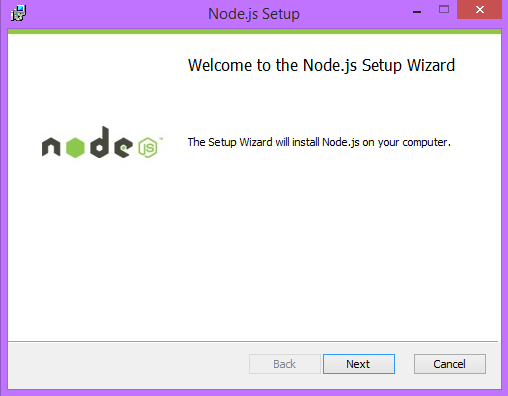
\includegraphics[width=10cm,height=15cm]{imagens/node1.png}
     \caption[NODEJS]{NODEJS.
     \textbf{Fonte: } Elaborado pelos autores.}
     \label{fig: nodejs}
\end{figure}

\begin{figure}[!htb]
     \centering
     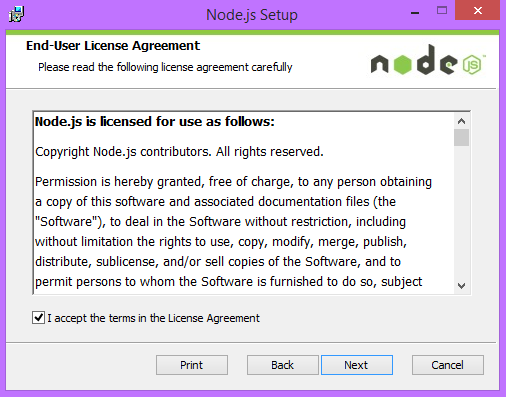
\includegraphics[width=10cm,height=8cm]{imagens/node2.png}
     \caption[NODEJS]{NODEJS.
     \textbf{Fonte: } Elaborado pelos autores.}
     \label{fig: nodejs}
\end{figure}

\begin{figure}[!htb]
     \centering
     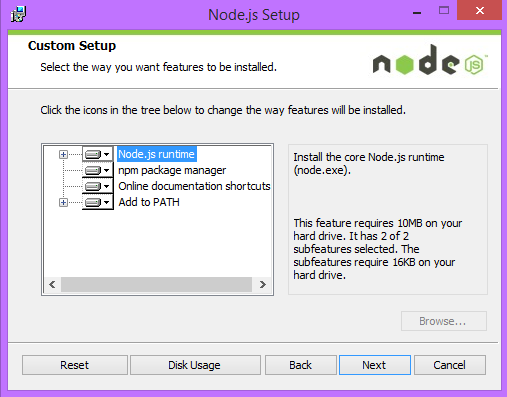
\includegraphics[width=10cm,height=9cm]{imagens/node3.png}
     \caption[NODEJS]{NODEJS.
     \textbf{Fonte: } Elaborado pelos autores.}
     \label{fig: nodejs}
\end{figure}

\begin{figure}[!htb]
     \centering
     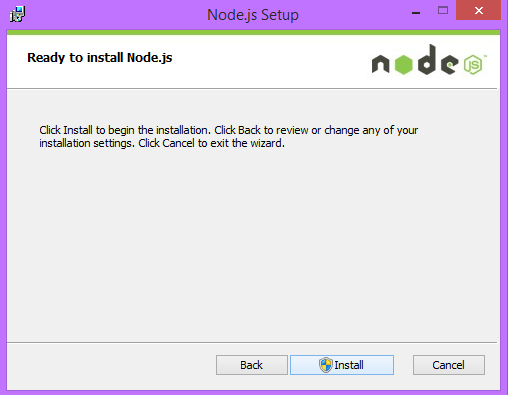
\includegraphics[width=10cm,height=8cm]{imagens/node4.png}
     \caption[NODEJS]{NODEJS.
     \textbf{Fonte: } Elaborado pelos autores.}
     \label{fig: nodejs}
\end{figure}

\begin{figure}[!htb]
     \centering
     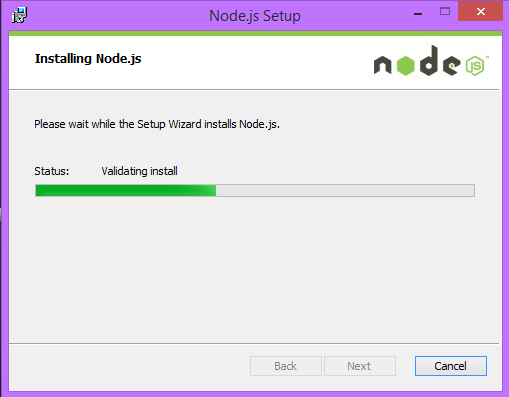
\includegraphics[width=10cm,height=8cm]{imagens/node5.png}
     \caption[NODEJS]{NODEJS.
     \textbf{Fonte: } Elaborado pelos autores.}
     \label{fig: nodejs}
\end{figure}

\begin{figure}[!htb]
     \centering
     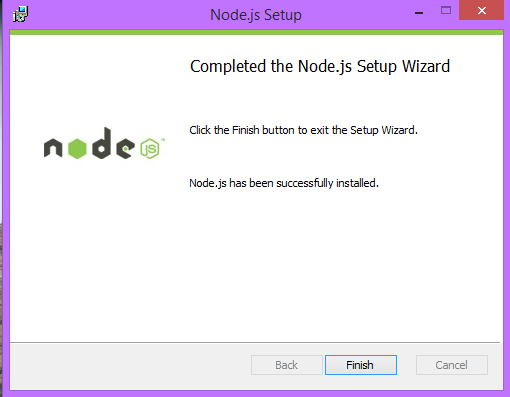
\includegraphics[width=10cm,height=8cm]{imagens/node6.png}
     \caption[NODEJS]{NODEJS.
     \textbf{Fonte: } Elaborado pelos autores.}
     \label{fig: nodejs}
\end{figure}
\end{comment}

%\clearpage
\newpage

\subsection{Instalação de dependências}


\par Para dar início ao desenvolvimento do projeto é necessário preparar o ambiente. Após ter instalado o \textit{NodeJS}, foi necessário instalar as dependências, utilizando o NPM \footnote{Node Package Manager}, para instalar as ferramentas que foram faladas no quadro teórico.

\par Abra o \textit{Prompt} de comando do S.O \footnote{Sistema Operacional} na pasta do projeto e digite \texttt{npm init}, conforme mostra Figura 1.


\begin{figure}[!htb]
    \caption[NPM init]{NPM init.
    
     \centering
     
     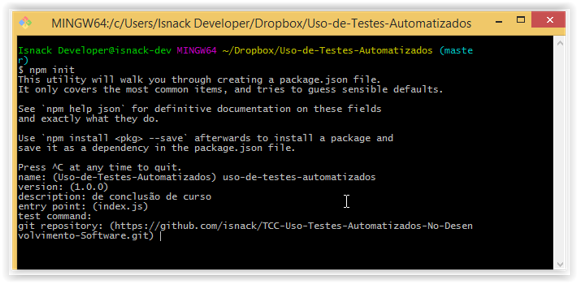
\includegraphics[width=12cm,height=10cm]{imagens/npm1.PNG}
     
     \textbf{Fonte: } Elaborado pelos autores.}
     \label{fig: npm init}
\end{figure}



\par É criado um arquivo \texttt{package.json}, este arquivo é responsável pelo gerenciamento das dependências do projeto e dos comandos dos testes que serão realizados posteriormente.

\par Abaixo a descrição dos campos que são requisitados para criação do arquivo \texttt{package.json}:

\begin{itemize}
 
 \item \texttt{Name}: Nome do Projeto.
 \item \texttt{Version}: Versão do Projeto.
 \item \texttt{Description}: Descrição do Projeto.
 \item \texttt{Entry Point}: Arquivo principal para inicializar o projeto.
 \item \texttt{Test Command}: Comando de testes. Nessa linha serão colocados comandos dos \textit{frameworks} que serão utilizados.
 \item \texttt{Git Repository}: Colocado o endereço do repositório do \textit{GitHub}.
 
\end{itemize}


\par Após os campos preenchidos é mostrado o esboço do arquivo que é gerado na pasta raiz do projeto, conforme mostra a Figura 2.

\begin{figure}[!htb]
    \caption[NPM ]{NPM.
    
     \centering
     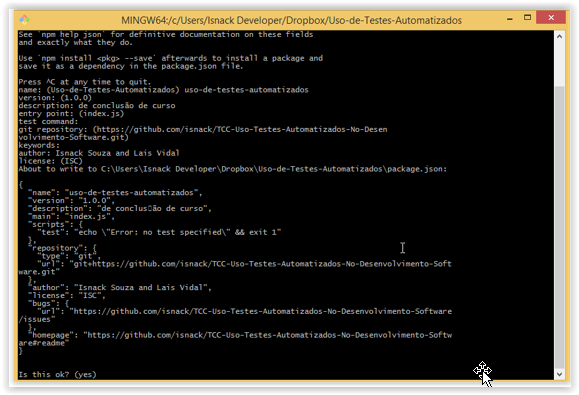
\includegraphics[width=12cm,height=10cm]{imagens/npm2.PNG}
     
     \textbf{Fonte: } Elaborado pelos autores.}
     \label{fig: npm}
\end{figure}


\par Após confirmar a criação, o arquivo é gerado na pasta do projeto, conforme mostra Figura 3.


\newpage
\begin{figure}[!htb]
    \caption[Arquivo Criado na Pasta ]{Arquivo Criado na Pasta.
     \centering
     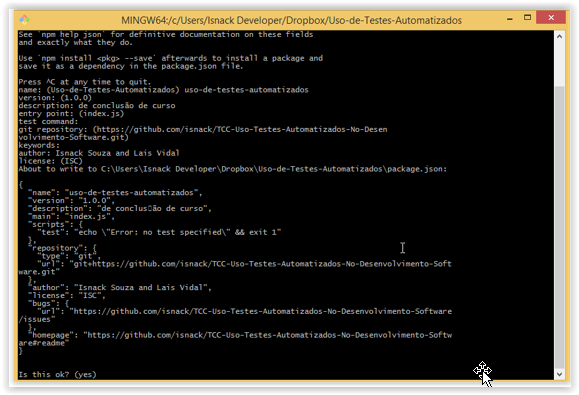
\includegraphics[width=12cm,height=8cm]{imagens/npm2.PNG}
     
     \textbf{Fonte: } Elaborado pelos autores.}
     \label{fig: Arquivo Criado na Pasta}
\end{figure}


\par Após inicializar o NPM é necessário executar os comandos de instalação dos pacotes das ferramentas \textit{CasperJS}, \textit{PhantomJS}, \textit{MochaJS} e \textit{ChaiJS}. Abaixo seguem os comandos que são executados:

\begin{itemize}
\item npm install casperjs -- save-dev
\item npm install phantomjs-prebuilt -- save-dev
\item npm install mocha chai  -- save-dev
\item npm install mongodb --save
\end{itemize}
\begin{figure}
  
  \caption[Exemplo de instalação das ferramentas ]{Exemplo de instalação das ferramentas.
     \centering
     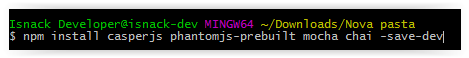
\includegraphics[scale=1]{imagens/npm4.PNG}
     
     \textbf{Fonte: } Elaborado pelos autores.}
     \label{fig: Exemplo de instalação das ferramentas}
\end{figure}



\newpage

\section{Testes}

\par Faz-se necessário a criação de uma pasta, nomeada \texttt{test}, para salvar os arquivos que são responsáveis pelos de testes, conforme mostra a Figura 5.

 \begin{figure}[!htb]
     \caption[Test ]{Test.
     \centering
     
     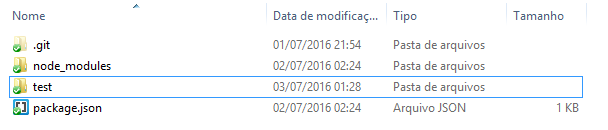
\includegraphics[scale=.75]{imagens/teste1.PNG}
     
     \textbf{Fonte: } Elaborado pelos autores.}
     \label{fig:test}
\end{figure}

\par Agora será criado um arquivo que executará os testes unitários, contendo o código fonte para cálculo do INSS.

\begin{comment}
 \begin{figure}[!htb]
     \caption[Teste Código Fonte ]{Teste Código Fonte.
     \centering
     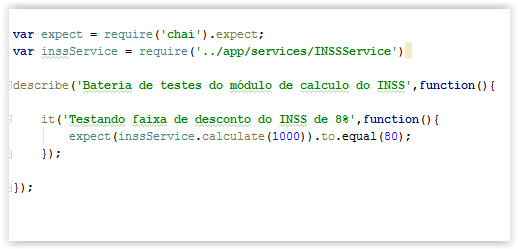
\includegraphics[width=12cm,height=8cm]{imagens/teste2.png}
     
     \textbf{Fonte: } Elaborado pelos autores.}
     \label{fig:teste código fonte}
\end{figure}
\end{comment}


\begin{lstlisting}[language=JavaScript, caption={[Teste de Código]{Teste de Código.  \textbf{Fonte:} Elaborado pelos autores.}}]
var expect = require('chai').expect;
var inssService = require('../app/services/INSSService')

describe('Bateria de teste do módulo de calculo do INSS',function(){
      it('Testando faixa de desconto do INSS de 8% ',function(){
        expect(inssService.calculate(1000).to.equal(80);
    });
});
\end{lstlisting}


\par A variável \texttt{expect} está recebendo os métodos do \textit{framework} \textit{Chai} que é responsável na execução dos testes, sua função é efetuar comparativo entre o valor de acordo com a regra especificada.

 \par A variável \texttt{inssService} recebe os serviços criados em arquivo, que é o módulo de cálculos. A função \texttt{describe}, descrita nas baterias de testes, e passada como parâmetro.
 
\par Foi necessário criar uma função padrão \texttt{it} na qual é feita uma descrição do teste a ser realizado (será testado a faixa de desconto de 8\%). Nessa função é utilizada a variável \texttt{expect} e o serviço \texttt{inssService} que é chamada de função \texttt{calculate} informando o salário bruto (1000), feito isso é chamado o método \texttt{.to.equal} informando o valor esperado (80). 

\par Definido o primeiro teste, roda-se o sistema para testar sua eficiência, e como não se tem os serviços implementados, é esperado mostrar um erro.

\par Ao executar os testes é necessário configurar um comando no arquivo \texttt{NPM} na linha de \textit{scripts}, basta adicionar o nome \texttt{test} passando o parâmetro \texttt{mocha}, conforme demonstra o Código 2.

\begin{comment}
 \begin{figure}[!htb]
     \caption[Configurar NPM - test ]{Configurar NPM - test.
     \centering
     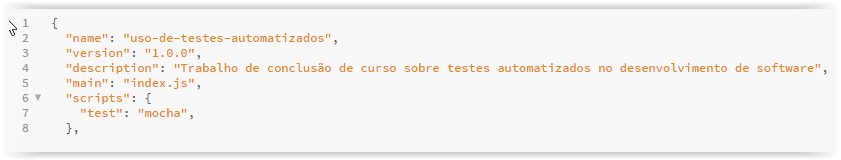
\includegraphics[width=12cm,height=8cm]{imagens/teste3.png}
    
     \textbf{Fonte: } Elaborado pelos autores.}
     \label{fig:configurar NPM - test}
\end{figure}
\end{comment}
 

\begin{lstlisting}[language=JavaScript, caption={[Configurar NPM test]{Configurar NPM test  \textbf{Fonte:} Elaborado pelos autores.}}]
{
"name": "uso-de-testes-automatizados",
"version": "1.0.0",
"description": "Trabalho de conclusão de curso sobre testes automatizados no desenvolvimento de software",
"main": "index.js",
"scripts": {
    "test": "mocha",
},
\end{lstlisting}



\par Após essa configuração abra o \textit{prompt} de comando dentro da pasta raiz do projeto, execute o comando \texttt{npm test} que executará o comando \textit{mocha}, conforme demonstra Figura 6.
 


\begin{figure}[!htb]
    \caption[NPM test ]{Npm test.
     \centering
     
     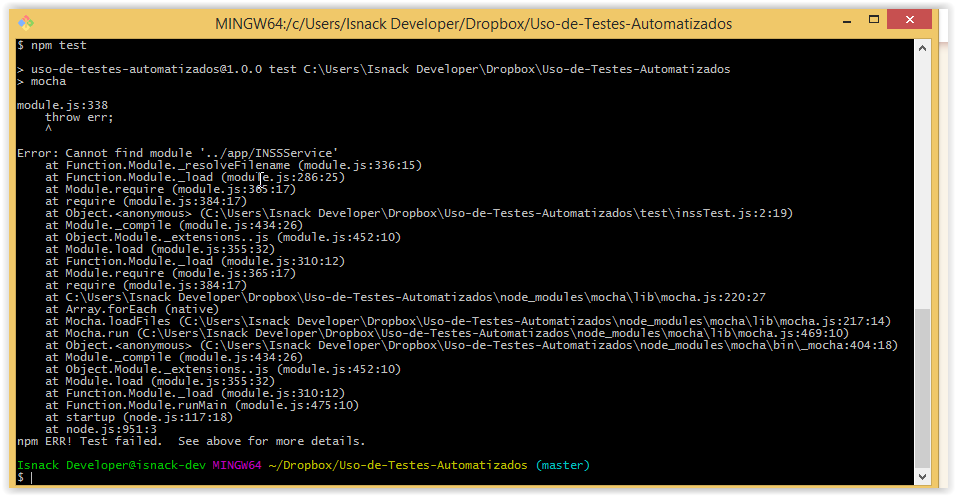
\includegraphics[scale=0.5]{imagens/teste4.png}
     
     \textbf{Fonte: } Elaborado pelos autores.}
     \label{fig:npm test}
\end{figure}

\newpage
\par O teste falhou porque não foi encontrado o módulo do INSS, para resolver isto, é necessário criar o módulo para o teste passar. Criado o módulo que foi salvo na pasta \texttt{services}, o método retornará o valor esperado e o objetivo é fazer o teste passar do jeito mais simples possível, a função retorna o valor 80, conforme mostra Código 3.

\begin{comment}
\begin{figure}[!htb]
     \caption[Modulo INSS ]{Modulo INSS.
     \centering
     
     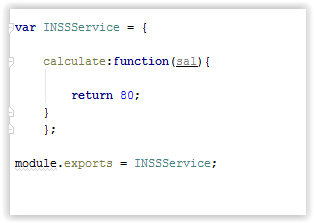
\includegraphics[width=12cm,height=8cm]{imagens/teste5.png}
    
     \textbf{Fonte: } Elaborado pelos autores.}
     \label{fig:modulo inss}
\end{figure}
\end{comment}


\begin{lstlisting}[language=JavaScript, caption={[Módulo INSS.]{Módulo INSS.  \textbf{Fonte:} Elaborado pelos autores.}}]
var INSSService = {

    calculate:function(sal){
       return 80;
   }
};
module.exports = INSSService;
\end{lstlisting}


\par Criado o serviço de cálculo com um retorno simples, roda-se o teste novamente para verificar se este erro passa.

\begin{figure}[!htb]
    \caption[Criação do primeiro teste INSS ]{Criação do primeiro teste INSS.
     \centering
     
     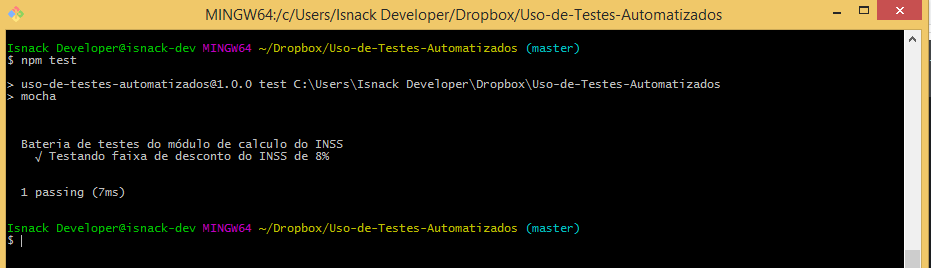
\includegraphics[scale=0.5]{imagens/teste6.png}
     
     \textbf{Fonte: } Elaborado pelos autores.}
     \label{fig:primeiro teste inss}
\end{figure}


\par Verifica-se que o teste passou conforme mostra Figura 7, após isso foram criados mais testes, conforme mostra Código 4, o objetivo é fazer os testes passarem, e assim, o código ser melhorado. Serão explicados todos os cenários que foram testados.

\begin{comment}
\begin{figure}[!htb]
    \caption[Criação de todos os testes INSS ]{Criação de todos os teste INSS.
     \centering
     
     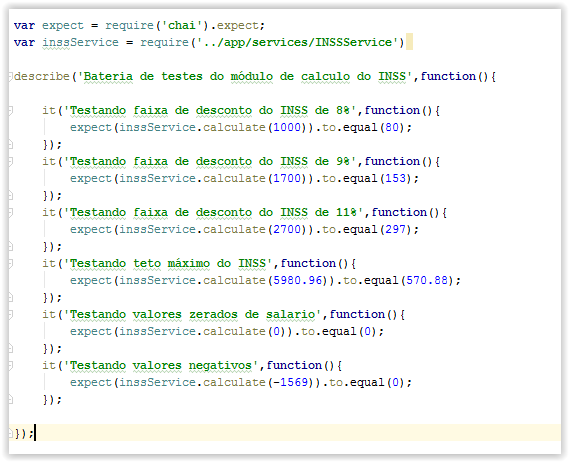
\includegraphics[width=12cm,height=8cm]{imagens/teste7.png}
     
     \textbf{Fonte: } Elaborado pelos autores.}
     \label{fig:todos teste inss}
\end{figure}
\end{comment}



\newpage

\begin{lstlisting}[language=JavaScript, caption={[Criação de todos os testes INSS.]{Criação de todos os testes INSS.  \textbf{Fonte:} Elaborado pelos autores.}}]
var expect = require('chai').expect;
var inssService = require('../app/services/INSSService');
describe('Bateria de testes do módulo de calculo do INSS',function(){    
    it('Testando faixa de desconto do INSS de 8%',function(){
        expect(inssService.calculate(1000)).to.equal(80);
    });
    it('Testando faixa de desconto do INSS de 9%',function(){
        expect(inssService.calculate(1700)).to.equal(153);
    });
    it('Testando faixa de desconto do INSS de 11%',function(){
        expect(inssService.calculate(2700)).to.equal(297);
    });
    it('Testando teto máximo do INSS',function(){
        expect(inssService.calculate(5980.96)).to.equal(570.88);
    });
    it('Testando valores zerados de salario',function(){
        expect(inssService.calculate(0)).to.equal(0);
    });
    it('Testando valores negativos',function(){
        expect(inssService.calculate(-1569)).to.equal(0);
    });
});

\end{lstlisting}

\par Os quatro primeiros cenários foram testadas as faixas de desconto do INSS de acordo com o MTPS – Ministério do Trabalho e Previdência Social, seguindo a tabela do ano vigente. 

\par Tabela para Empregado, Empregado Doméstico e Trabalhador Avulso.



\begin{figure}[!htb]
     \caption[Tabela INSS ]{Tabela INSS.
     \centering
     
     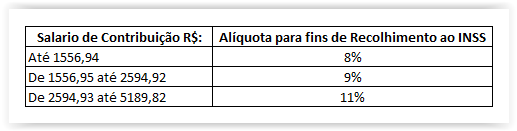
\includegraphics[width=8.89cm,height=2.75cm]{imagens/inss.png}
    
     \textbf{Fonte: } Elaborado pelos autores.}
     \label{fig:tabela inss}
\end{figure}




\par Nos últimos cenários foram testados valores com zero e negativo, deve retornar 0 para efeitos de cálculo. No Código 5 é mostrado o código do serviço pronto e os testes passando.

\begin{comment}

\begin{figure}[!htb]
     \caption[INSS Service ]{INSS Service.
     
     \centering
     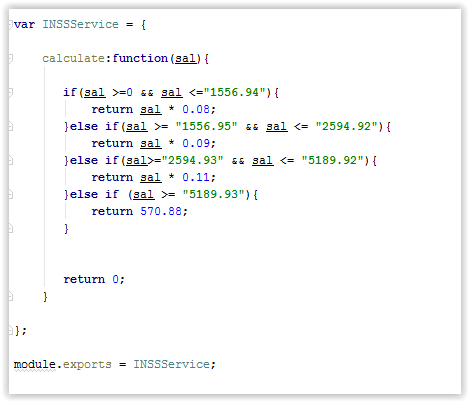
\includegraphics[width=12cm,height=8cm]{imagens/teste8.png}
    
     \textbf{Fonte: } Elaborado pelos autores.}
     \label{fig:INSS Service}
\end{figure}

\end{comment}

\newpage
\begin{lstlisting}[language=JavaScript, caption={[INSS Service.]{INSS Service.  \textbf{Fonte:} Elaborado pelos autores.}}]
var INSSService = {
        calculate:function(sal){
           if(sal >=0 && sal <="1556.94"){
              return sal * 0.08;
           }else if(sal >= "1556.95" && sal <= "2594.92"){
               return sal * 0.09;
           }else if(sal>="2594.93" && sal <= "5189.92"){
               return sal * 0.11;
           }else if (sal >= "5189.93"){
               return 570.88;
       }
         return 0;
    }
};
module.exports = INSSService;

\end{lstlisting}


\par Todos os testes que foram criados para o INSS, com suas respectivas faixas salariais, seus descontos e com valor negativo e zerado, mostrando que os testes passaram em todos os requisitos, conforme mostra a Figura 9.

\begin{figure}[!htb]
    \caption[Testes INSS Passando ]{Testes INSS Passando.
     \centering
     
     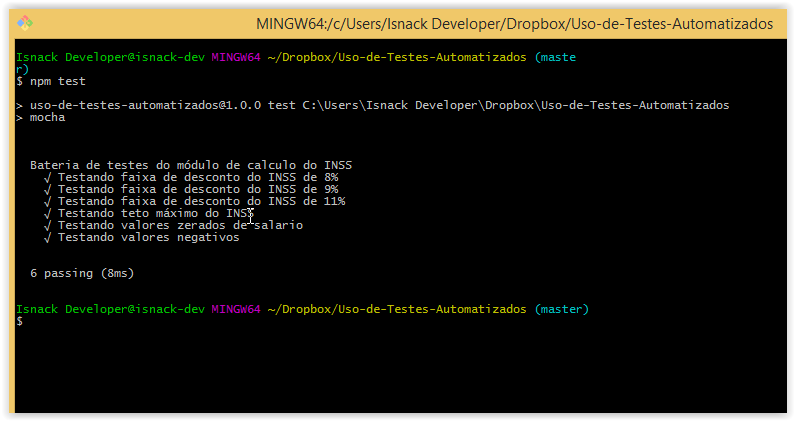
\includegraphics[scale=0.5]{imagens/teste9.png}
     
     \textbf{Fonte: } Elaborado pelos autores.}
     \label{fig:testes inss passando}
\end{figure}


\par Criado um arquivo que executará os testes unitários, que contém o código fonte para calculo do IR.
 
\begin{comment}
 \begin{figure}[!htb]
    \caption[Testes IR  ]{Testes IR.
     \centering
     
     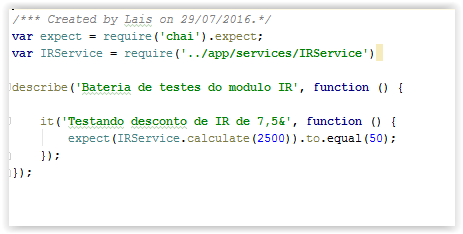
\includegraphics[width=12cm,height=8cm]{imagens/teste17.png}
     
     \textbf{Fonte: } Elaborado pelos autores.}
     \label{fig:testes ir}
\end{figure}
\end{comment}

\newpage

\begin{lstlisting}[language=JavaScript, caption={[IR Service.]{IR Service.  \textbf{Fonte:} Elaborado pelos autores.}}]
var expect = require('chai').expect;
var IRService = require('../app/services/IRService');

describe('Bateria de testes do Módulo IR',function(){
       it('Testando desconto de IR de 7,5%',function(){
       expect(IRService.calculate(2500)).to.equal(50);
    });
});

\end{lstlisting}



\par Abra o \textit{prompt} de comando, digite o comando \texttt{npm test}, o teste não irá passar, pois o valor esperado não é o correto, conforme mostra a Figura 10.

 \begin{figure}[!htb]
    \caption[Teste IR dando erro ]{Teste IR dando erro.
     \centering
     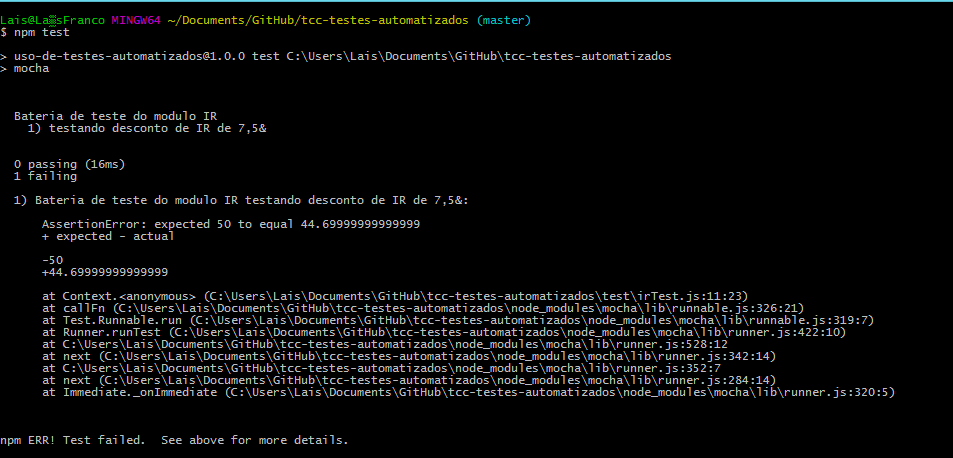
\includegraphics[scale=0.5]{imagens/teste16.png}
     
     \textbf{Fonte: } Elaborado pelos autores.}
     \label{fig:teste ir dando erro}
\end{figure}


\par Atualizando o valor esperando pela variável \texttt{to.equal}.



\begin{lstlisting}[language=JavaScript, caption={[Teste IR.]{Teste IR.  \textbf{Fonte:} Elaborado pelos autores.}}]
var expect = require('chai').expect;
var IRService = require('../app/services/IRServices');

describe('Bateria de teste do módulo IR', function(){
        it('Testando desconto de IR de 7,5%', funciton(){
        expect(IRService.calculate(2500)).to.equal(44,699999999999);
    });
});

\end{lstlisting}
\begin{comment}


 \begin{figure}[!htb]
     \caption[Teste Ir dando erro ]{Teste IR dando erro.
     \centering
     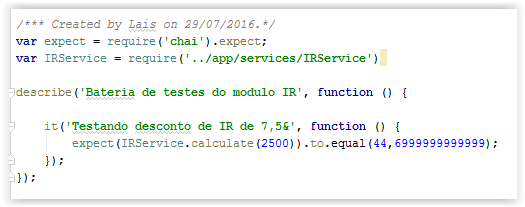
\includegraphics[width=12cm,height=6cm]{imagens/teste10.png}
    
     \textbf{Fonte: } Elaborado pelos autores.}
     \label{fig:teste ir dando erro}
\end{figure}
\end{comment}
\newpage

\par Após o valor atualizado o teste irá passar, conforme mostra a Figura 11.

\begin{figure}[!htb]
     \caption[NPM test - IR ]{NPM test - IR.
     \centering
     \raggedleft
     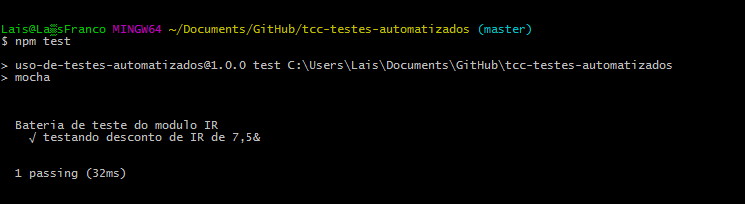
\includegraphics[scale=.70]{imagens/teste11.png}
    \centering
     \textbf{Fonte: } Elaborado pelos autores.}
     \label{fig:npm test - ir}
\end{figure}


\par Os quatro primeiros cenários foram testadas as faixas de desconto do IR de acordo com a tabela do ano vigente.


\begin{lstlisting}[language=JavaScript, caption={[Criação de todos os testes IR.]{Criação de todos os testes IR.  \textbf{Fonte:} Elaborado pelos autores.}}]
var expect = require('chai').expect;
var IRService = require('../app/services/IRService');
describe('Bateria de testes do modulo IR', function () {
         it('Testando desconto de IR de 7,5%', function () {
          expect(IRService.calculate(2500)).to.be.closeTo(44.70,0.01);
      });
         it('Testando desconto de IR de 15%', function () {
            expect(IRService.calculate(3500)).to.equal(170.20);
     });
        it('Testando desconto de IR de 22,5%', function () {
         expect(IRService.calculate(4500)).to.equal(376.37);
     });
         it('Testando desconto de IR de 27,5%', function () {
          expect(IRService.calculate(5500)).to.be.closeTo(643.14,0.01);
     });
         it('Testando valor de IR negativo', function () {
          expect(IRService.calculate(-1979)).to.equal(0);
     });
         it('Testando valores zerados', function () {
          expect(0).to.equal(IRService.calculate(0));
     });
});

\end{lstlisting}
\begin{comment}


 \begin{figure}[!htb]
    \caption[Criação de todos os testes IR ]{Criação de todos os testes IR.
     \centering
     
     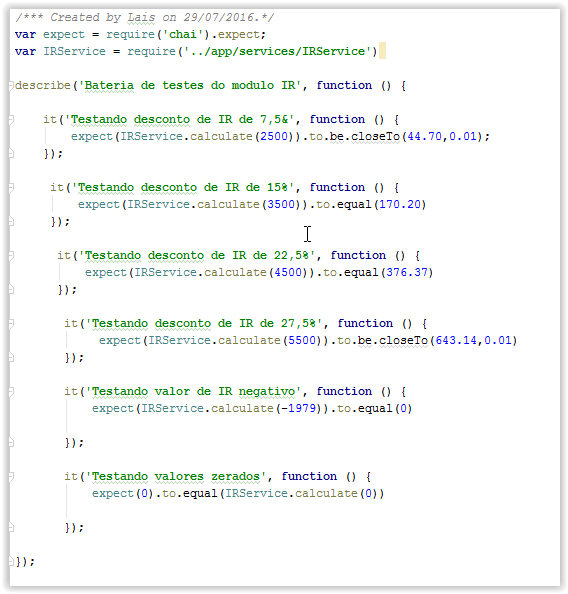
\includegraphics[width=12cm,height=10cm]{imagens/teste13.png}
     
     \textbf{Fonte: } Elaborado pelos autores.}
     \label{fig:criação de todos os testes INSS}
\end{figure}
\end{comment}

\newpage
\par  Foi utilizado nesse teste a função de comparação de resultados \texttt{to.be.closeTo}, nessa função é informado o valor que se deseja comparar com um intervalo de tolerância no resultado, que no caso é de 0.01.

\par Tabela de desconto do Imposto de Renda retido na fonte.

 \begin{figure}[!htb]
    \caption[Tabela IR ]{Tabela IR.
     \centering
     
     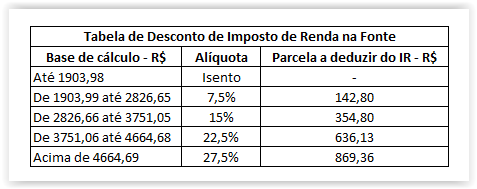
\includegraphics[width=12cm,height=6cm]{imagens/IR.png}
     
     \textbf{Fonte: } Elaborado pelos autores.}
     \label{fig:tabela ir}
\end{figure}

\par Os últimos cenários foram testados valores com zero e negativo, deve retornar 0 para efeitos de cálculo. No Código 9 é mostrado o código do serviço pronto e os testes passando.

\begin{comment}


\begin{figure}[!htb]
    \caption[IrService ]{IrService.
     \centering
     
     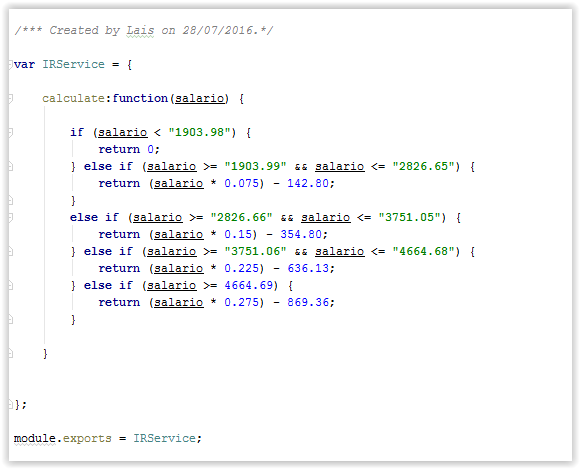
\includegraphics[width=12cm,height=6cm]{imagens/teste50.PNG}
     
     \textbf{Fonte: } Elaborado pelos autores.}
     \label{fig:modulo irService}
\end{figure}
\end{comment}


\begin{lstlisting}[language=JavaScript, caption={[IR Service.]{IR Service.  \textbf{Fonte:} Elaborado pelos autores.}}]
var IRService = {
    calculate:function(salario) {
        if (salario < "1903.98") {
            return 0;
        } else if (salario >= "1903.99" && salario <= "2826.65") {
            return (salario * 0.075) - 142.80;
        }
        else if (salario >= "2826.66" && salario <= "3751.05") {
            return (salario * 0.15) - 354.80;
        } else if (salario >= "3751.06" && salario <= "4664.68") {
            return (salario * 0.225) - 636.13;
        } else if (salario >= 4664.69) {
            return (salario * 0.275) - 869.36;
        }}
};
module.exports = IRService;

\end{lstlisting}

\newpage
\par Todos os testes que foram criados para o IR, com suas respectivas faixas salariais, seus descontos e com valor negativo e zerado, mostrando que os testes passaram em todos os requisitos, conforme mostra a Figura 13.

\begin{figure}[!htb]
    \caption[Teste de Ir Passando ]{Teste de Ir Passando.
     \centering
     
     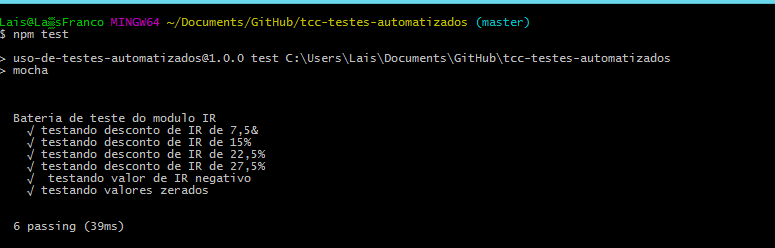
\includegraphics[width=12cm,height=8cm]{imagens/teste15.png}
     
     \textbf{Fonte: } Elaborado pelos autores.}
     \label{fig:teste de IR passando}
\end{figure}

 \par Criado os módulos de cálculo do desconto do INSS e do Imposto de Renda e devidamente testados, fez-se necessário a criação do módulo que calcula o salário líquido. Mas primeiro deve-se criar os testes.
\par Foi criado um arquivo nomeado \texttt{intergrationTestInssIr} dentro da pasta \texttt{test}, que é responsável pela realização dos testes de integração (INSS e IR), conforme mostra a Figura 14, a criação desse arquivo.
 
 
 \begin{figure}[!htb]
    \caption[Criação do arquivo para teste de integração ]{Criação do arquivo para teste de integração.
     \centering
     
     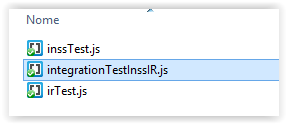
\includegraphics[scale=1.5]{imagens/teste18.png}
     
     \textbf{Fonte: } Elaborado pelos autores.}
     \label{fig:criação do arquivo para teste de integração}
\end{figure}

 \newpage
 \par O primeiro teste visa verificar um valor que possua desconto do INSS e não seja possível realizar o desconto do Imposto de renda (sendo o salário bruto 1500, o resultado esperado com o desconto de INSS é de 1380), conforme mostra Código 10.
 


 \begin{lstlisting} [language=JavaScript, caption={[ Primeiro teste de integração.]{ Primeiro teste de integração. \textbf{Fonte:} Elaborado pelos autores.}}]
var expect = require('chai').expect;
var IRService = require('../app/services/SalarioLiquidoService');
describe('Testa se os descontos de cada serviço está como especificado',function () {
            
   it('Salario faixa minima na qual é descontado somente o INSS', function () {
     expect(salarioLiquidoService.calculate(1500)).to.equal(1380);
    });         
});

\end{lstlisting}

\begin{comment}
 \begin{figure}[!htb]
     \caption[Primeiro teste de integração ]{Primeiro teste de integração.
     \centering
     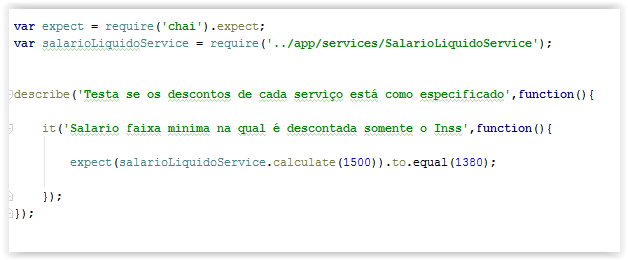
\includegraphics[width=12cm,height=6cm]{imagens/teste19.png}
    
     \textbf{Fonte: } Elaborado pelos autores.}
     \label{fig:primeiro teste de integração}
\end{figure}
\end{comment}


\par Executado o teste, verificou-se que, conforme o esperado, o teste falhou, pois não foi criado o serviço chamado \texttt{salarioLiquidoService}, conforme mostra Figura 15.

\begin{figure}[!htb]
    \caption[Teste falhando ]{Teste falhando.
     \centering
     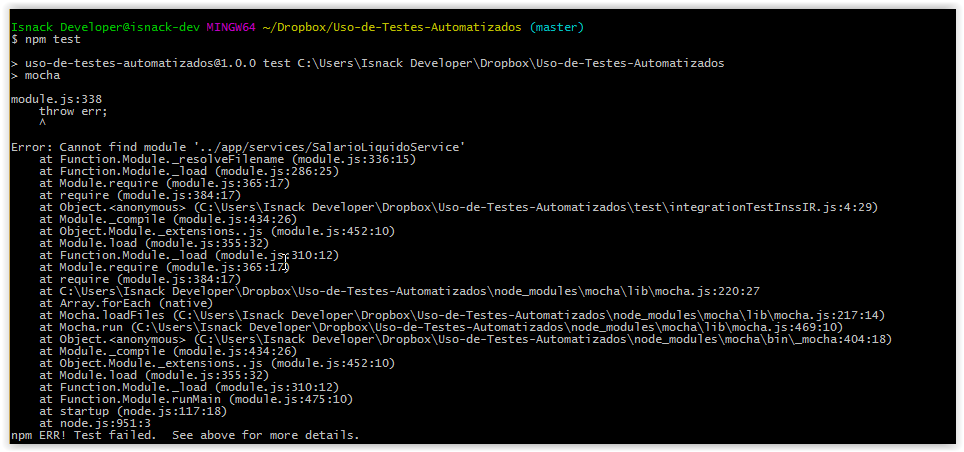
\includegraphics[scale=0.5]{imagens/teste20.png}
     
     \textbf{Fonte: } Elaborado pelos autores.}
     \label{fig:teste falhando}
\end{figure}


\par Após realizar o primeiro teste, foi criado o módulo para calcular o salário liquido dentro da pasta \texttt{services}, seguindo a mesma metodologia dos testes anteriores de criar uma solução simples e depois refatorar, ou seja, melhorar o código. O Código 11 faz essa demonstração.

\newpage


 
\begin{lstlisting}[language=JavaScript, caption={[Módulo de salário líquido.]{Módulo de salário líquido. \textbf{Fonte:} Elaborado pelos autores.}}]
var  IRService = require('./IRService');
var INSSService = require('./INSSService');

var SalarioLiquidoService = {
  calculate:function (salario) {

    var salarioBruto = salario;
    var valorDescontadoInss,salarioComDescontoInss,
        valorDescontadoIR,salarioLiquido;
    
    valorDescontadoInss = INSSService.calculate(salarioBruto);
    salarioComDescontoInss = salarioBruto - valorDescontadoInss;
    valorDescontadoIR = IRService.calculate(salarioComDescontoInss);
    salarioLiquido = salarioComDescontoInss - valorDescontadoIR;

   return salarioLiquido;
}};
module.exports =  SalarioLiquidoService;
\end{lstlisting}

\begin{comment}
\begin{figure}[!htb]
     \caption[Código do módulo de salário liquido ]{Código do módulo de salário liquido.
     \centering
     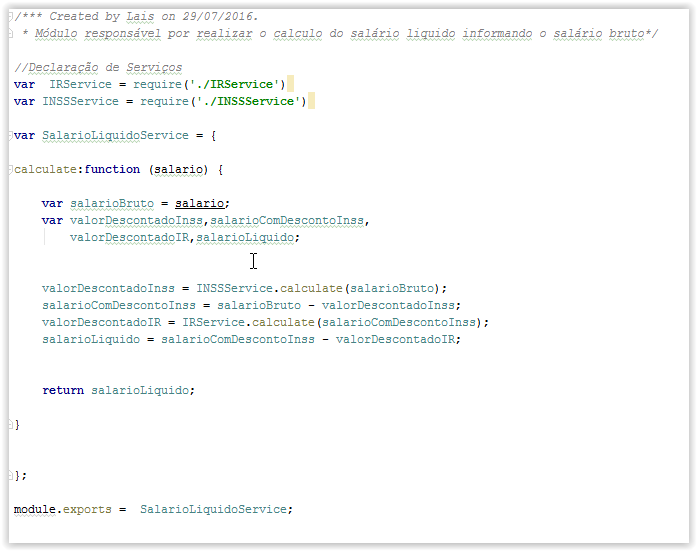
\includegraphics[width=12cm,height=6cm]{imagens/teste21.png}
     
     \textbf{Fonte: } Elaborado pelos autores.}
     \label{fig:código do módulo de salário liquido}
\end{figure}
\end{comment}

\par O módulo recebe o valor do salário bruto como parâmetro, em seguida é atribuído a variável, é chamada de \texttt{salarioBruto}, são criadas outras variáveis: \texttt{valorDescontadoInss}, \texttt{salarioComDescontoInss}, \texttt{valorDescontadoIR} e \texttt{salarioLiquido}.

\par A variável \texttt{valorDescontadoINSS} recebe como resultado o módulo de cálculo do desconto do INSS, e a variável \texttt{salarioComDescontoINSS} recebe o valor de  cálculo do salário bruto menos o desconto do INSS, \texttt{valorDescontadoIR} recebe como resultado o módulo de cálculo do Imposto de Renda e o \texttt{salarioLiquido} recebe o resultado final do salário menos os descontos de INSS e Imposto de Renda.

\par O teste foi executado novamente, conforme mostra a Figura 16.
\newpage
\begin{figure}[!htb]
      \caption[Teste de integração sendo rodado novamente ]{Teste de integração sendo rodado novamente.
     \centering
     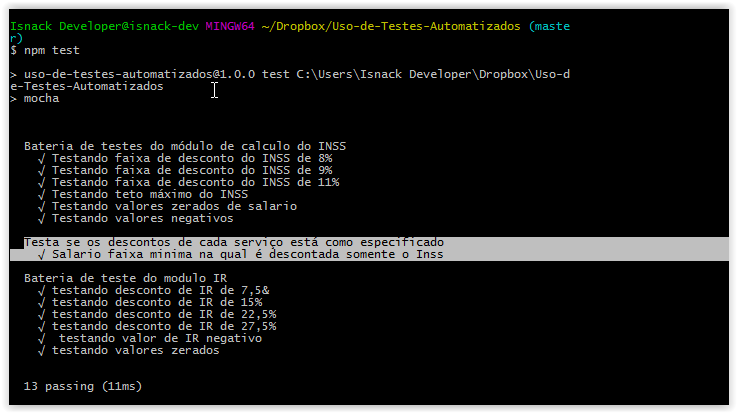
\includegraphics[scale=0.5]{imagens/teste22.png}
   
     \textbf{Fonte: } Elaborado pelos autores.}
     \label{fig:teste de integração sendo rodado novamente}
\end{figure}


\par Passando o primeiro teste foram criados outros testes para verificar se a integração entre as unidades de cálculo de desconto do INSS e do Imposto de Renda estavam corretas.


  \par As condições usadas para fazer os outros testes:
\begin{enumerate}

 \item Verificar se colocar um salário que não possua desconto do Imposto de Renda, com isso foi possível verificar se o módulo de Imposto de Renda poderia afetar o cálculo do salário líquido. Conforme mostra o Código 12.
 
  \item Fazer a verificação se o módulo realizou o desconto de 9\% do INSS e de 7,5\% do Imposto de Renda.
  \item Fazer a verificação se o módulo realizou o desconto de 11\% do INSS e 15\% do Imposto de Renda.
  \item Fazer a verificação se o módulo realizou o desconto de 11\% do INSS e 22,5\% do Imposto de Renda.
  \item Fazer a verificação se o módulo realizou o desconto do teto \end{enumerate}
  
\newpage
 
\begin{lstlisting} [language=JavaScript, caption={[ Todos os testes do salário líquido.]{ Todos os testes do salário líquido.  \textbf{Fonte:} Elaborado pelos autores.}}]
var expect = require('chai').expect;
var salarioLiquidoService = require('../app/services/SalarioLiquidoService');

describe('Testa se os desconto de cada servico está como especificado',function(){
    
it('Faixa minima na qual é descontada somente o Inss',function(){
  expect(salarioLiquidoService.calculate(1500)).to.equal(1380);
});
it('Faixa 9% de desconto do Inss com desconto de IR faixa de 7.5%',function(){
  expect(salarioLiquidoService.calculate(2300)).to.be.closeTo(2078.83,0.01);
});
it('Faixa 11% de desconto do Inss com desconto de IR faixa de 15%',function(){
  expect(salarioLiquidoService.calculate(3200)).to.be.closeTo(2775.60,0.01);
});
it('Faixa 11% de desconto do Inss com desconto de IR faixa de 22,5%',function(){
   expect(salarioLiquidoService.calculate(4450.00)).to.be.closeTo(3705.52,0.01);
});
it('Desconto teto do Inss com desconto de IR faixa de 27,5%',function(){
 expect(salarioLiquidoService.calculate(5200.00)).to.be.closeTo(4223.70,0.01)
});    
});    
    
    
\end{lstlisting}
\begin{comment}
\begin{figure}[!htb]
     \caption[Todos os Teste do salário liquido ]{Todos os Teste do salário liquido.
     \centering
     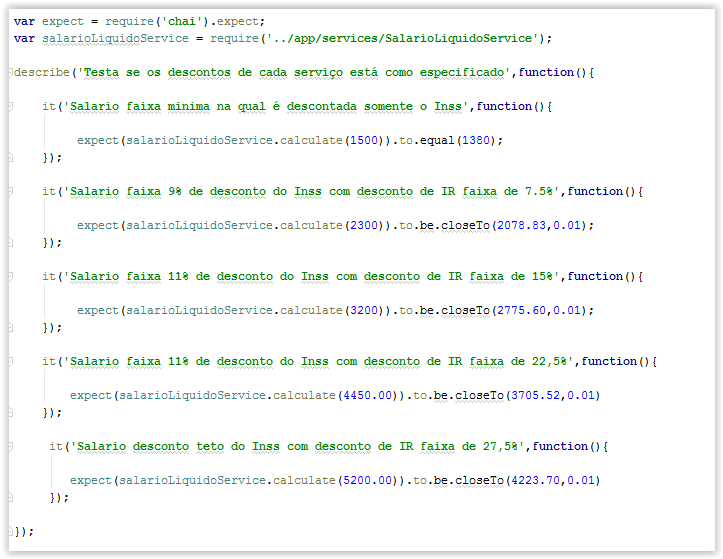
\includegraphics[width=12cm,height=6cm]{imagens/teste23.png}
     
     \textbf{Fonte: } Elaborado pelos autores.}
     \label{fig:todos os Teste do salário liquido}
\end{figure}
\end{comment}

\par Nesse teste foi utilizado a função de comparação de resultados \texttt{to.be.closeTo}, nessa função é informado o valor que se deseja comparar com um intervalo de tolerância no resultado, que no caso é de 0.01.

\par Com os testes de unidade e integração prontos, a próxima etapa foi a realização dos testes funcionais. Foi necessário a criação do modelo de banco de dados utilizando o \textit{MongoDB} e a configuração dos serviços em \textit{RestApi} e depois a criação das páginas \textit{web}.

\newpage
\par Primeiramente foi criado a estrutura para guardar os dados no \textit{MongoDB} e, portanto foi utilizado o \textit{mongoose} para criar essa estrutura, conforme mostra o Código 13.



\begin{lstlisting}[language=JavaScript, caption={[Estrutura Documento MongoDB.]{Estrutura Documento MongoDB.  \textbf{Fonte:} Elaborado pelos autores.}}]
var mongoose = require('mongoose');
var funcionarioSchema = new mongoose.Schema({
  nome: String,
  endereco: String,
  cidade: String,
  estado: String,
  bairro: String,
  salario:Number
 });

\end{lstlisting}

\par Com essa estrutura é possível guardar os seguintes dados:
 \begin{itemize}
  \item Nome;
  \item Endereço;
  \item Cidade;
  \item Estado;
  \item Bairro;
   \item Salário.
 \end{itemize}

\par Para o servidor \textit{Rest} foi utilizado o \textit{framework Restify} com as seguintes rotas:
\begin{itemize}
 \item \textbf{Contexto da aplicação:} \url{http://<endereço_servidor/<rota>};
 
 \item \textbf{api/funcionarios:} obter lista de funcionários via \textit{get};
 
\item \textbf{api/folhaSal/:id:} Obter folha salarial por id do funcionário via \textit{get};

\item \textbf{api/funcionarios/:id:} obter funcionário específico por id via \textit{get};

\item \textbf{api/funcionários:}  Enviar registro de funcionários via \textit{post};

\item \textbf{api/funcionarios:} Atualizar registro de funcionário via \textit{put};

\item \textbf{api/funcionarios/:id:} Deletar funcionário via \textit{delete};

\item \textbf{api/authentication:} Realizar autenticação de usuário via \textit{post}.

\end{itemize}

\par Para a criação das páginas foi utilizado o \textit{Bootstrap} e o \textit{AngularJS} e atribuiu-se as seguintes responsabilidades:
\begin{itemize}
 \item Autenticar;
 \item Listar Funcionários;
 \item Adicionar Funcionário;
 \item Gerar Folha de Pagamento.
\end{itemize}

\par As páginas utilizam esses serviços que foram citados anteriormente, com tudo isso pronto inicia-se a criação dos testes funcionais.

\par Para a criação dos testes funcionais foi utilizado o \textit{framework CasperJS}, o qual já foi demonstrada sua instalação anteriormente.


\par Primeiramente é criado o arquivo de teste na pasta \texttt{test}, mas ao rodar os testes unitários o \textit{mocha} acabava rodando os testes do \textit{CasperJS}, pois o \textit{mocha} não é preparado para rodar o \textit{CasperJS}, para resolver esse problema foi necessário criar uma pasta somente para os testes funcionais.

\par Criado um roteiro para testar toda a aplicação, na qual consiste em simular o usuário acessando o sistema, fazendo o login
com dados incorretos e depois com dados corretos, verificando se o sistema dá o retorno para o usuário de que algo está errado ou ocorreu algum problema.

\par Depois de verificar se a página que ele está dando acesso é a correta, no qual deverá aparecer a lista de funcionários, depois adicionar um novo funcionário, gerar folha de pagamento do mesmo, podendo atualizar esse cadastro e por último fazer sua exclusão. Com esse roteiro é iniciado a criação do \textit{script} que executam os testes


\par Dentro do projeto foi criado uma pasta denominada \texttt{testFunctional}, e dentro dessa pasta foi criado o arquivo \texttt{functionalTest.js}. Foi necessário criar uma função \texttt{casper.test\\.begin} para iniciar os testes, essa função tem como parâmetros o nome da bateria de testes e a quantidade de testes que serão realizados.

\par Para começar o teste precisa realizar a autenticação, para isso foi criado um método para realizar esse procedimento, no Código 14, como pode ser observado, primeiro é feito a chamada do método do objeto formulário \texttt{testAutenticacao}, e passado a instância do \textit{CasperJS} que é a variável \texttt{casper}, esse método tem como responsabilidade realizar o teste de autenticação de usuário.

\newpage
\begin{lstlisting}[language=JavaScript, caption={[Chamada da função para o teste de autenticação.]{Chamada da função para o teste de autenticação. \textbf{Fonte:} Elaborado pelos autores.}}]
casper.test.begin('Teste Funcional da Folha de Pagamento', 15, function (test) {
       formulario.testAutenticacao(casper);
}

\end{lstlisting}

\par No Código 15 primeiro é chamado o método \texttt{casper.start} que é responsável em acessar a aplicação \textit{web}, informando uma url na qual a aplicação está sendo executada.



\begin{lstlisting}[language=JavaScript, caption={[Acessar aplicação utilizando método casper.start.]{Acessar aplicação utilizando método casper.start.  \textbf{Fonte:} Elaborado pelos autores.}}]
testAutenticacao:function(casper){
        casper.start('http://localhost:8585/public/');
            casper.then(function (casper) {
                this.test.assertExists(x('//*[@id="botao"]'), 'Testando se existe o botão de login');
        });
            casper.then(function () {
                 this.click(x('//*[@id="botao"]'));
         });
}
\end{lstlisting}

\par O método \texttt{test.assertExists} testa se existe um elemento que é especificado, e a variável \texttt{x} é uma instância para o \textit{CasperJS} entender o \textit{XPath} e sua instanciação é feita no começo do \textit{script}, como demonstra o Código 16.


\begin{lstlisting}[language=JavaScript, caption={[Atribuição para o seletor de XPath.]{Atribuição para o seletor de XPath.  \textbf{Fonte:} Elaborado pelos autores.}}]
var x = require('casper').selectXPath;

\end{lstlisting}


\par Feito essa instanciação, o teste é capaz de selecionar elementos via \textit{XPath} para selecionar o elemento utilizando \textit{XPath} basta carregar a página desejada, apertar o botão F12 do teclado, selecionar a aba \textit{elements}, clicar com o botão direito em cima do elemento e depois selecionar a opção \textit{copy} e em seguinda \textit{copy XPath}, conforme mostra a Figura 17, esse processo é feito em todos os elementos necessários para realização do teste.


\newpage

\begin{figure}[!htb]

     \caption[Copiar o XPath ]{Copiar o XPath.
     
     \raggedleft
      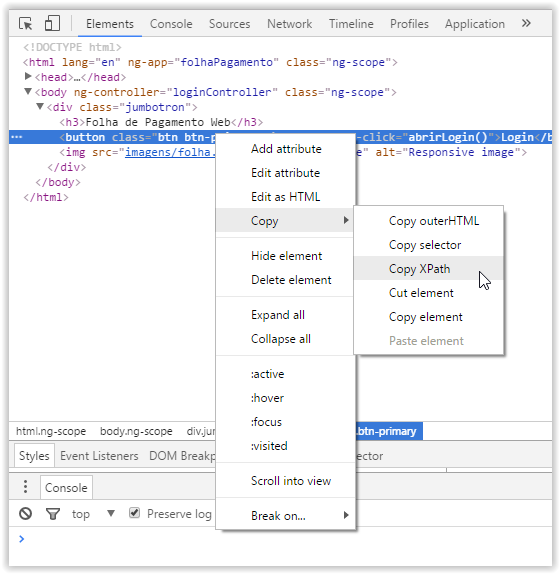
\includegraphics[width=15cm,height=20cm]{imagens/teste51.PNG}
   \centering
     \textbf{Fonte: } Elaborado pelos autores.}
     \label{fig:Copiar o XPath}
\end{figure}

\newpage

\par Com o \textit{XPath} selecionado o método \texttt{test.assertExists} verifica se existe o elemento com a identificação \texttt{*[@id="botao"]}.

\par Os procedimentos do teste ficam dentro do método \texttt{casper.then}, esse método adiciona um passo que o \textit{script} deve fazer, então é chamado o método \texttt{click} e nesse método é informado o \textit{XPath} do botão de \textit{login}, assim, possibilita o acesso à página de login, como pode ser observado no Código 15.

\par Na página de \textit{login} é necessário informar usuário e senha, para o \textit{script} fazer isso é necessário chamar o método \texttt{sendKeys} e informar o elemento que é desejado e no outro parâmetro a informação, que nesse caso o usuário é "admin".


\begin{lstlisting}[language=JavaScript, caption={[Teste que verifica a validação da página.]{Teste que verifica a validação da página. \textbf{Fonte:} Elaborado pelos autores.}}]
casper.then(function () {
    this.sendKeys('#usuario', 'admin');
});
casper.then(function () {
    this.capture('testFunctional/img/teste3.png');
});
casper.then(function () {
    this.test.assertTextExists('Por favor, preencha os campos!', 'Testando se no corpo da pagina contém a frase "Por favor, preencha os campos!"');
});
\end{lstlisting}

\par Segundo o teste, informar somente o \textit{login} e verificar se a página exibe a informação "Por favor, preencha os campos!", esse teste está verificando a validação do formulário e se está funcionando corretamente. Para realizar o teste é chamando o método \texttt{test.assertTextExists} e a sua função é testar se o texto "Por favor, preencha os campos!" foi exibido na página ou se está no corpo da página como exemplifica o Código 17.

\par Para auxiliar na produção do teste a função \texttt{capture} auxilia a fazer um \textit{debug} no teste, possibilitando assim, visualizar após a execução do teste como a página estava no momento que foi executado o procedimento.


\par Depois foi informado a senha errada, o \textit{script} clica no botão enviar utilizando o método \texttt{click} passando o \textit{XPath} especificado no botão.

\newpage

\begin{lstlisting}[language=JavaScript, caption={[Teste que verifica a validação da página novamente.]{Teste que verifica a validação da página novamente.  \textbf{Fonte:} Elaborado pelos autores.}}]
casper.then(function () {
    this.sendKeys('#senha', 'admin1');
    this.click(x('//*[@id="loginForm"]/div[5]/div/button'));
});
casper.wait(3000, function () {
    this.echo("Esperando Resposta do Servidor!!");
});
casper.then(function () {
    this.test.assertTextExists('Usuario e/ou senha inválidos','Testando se o usuário foi impedido de entrar e se a mensagem de alerta é a correta"');
});

\end{lstlisting}

\par O teste verifica se a informação "Usuario e/ou senha inválidos" foi exibido, utilizando o método \texttt{test.assertTextExists}, no qual testa a condição do Código 18. Outra função importante é o \texttt{wait}, nela tem a possibilidade de colocar um tempo de espera em milissegundos no teste que será executado, pois em vários casos a página que está sendo testada carrega em menor velocidade que o processamento do teste, sendo necessário utilizar essa função.


\begin{lstlisting}[language=JavaScript, caption={[Teste que verifica o título da página.]{Teste que verifica o título da página.  \textbf{Fonte:} Elaborado pelos autores.}}]
casper.then(function () {
  this.test.assertTitle("Funcionários", "Testando se está na página de Funcionários");      
});

\end{lstlisting}

\par No ultimo teste são informados os dados corretos e é testado se o título da página é "Funcionários". Para realizar esse teste foi utilizado o método \texttt{test.assertTitle} informando o título desejado. Com isso se compara o título processado na página, como exemplifica o Código 19.

\par Outro teste realizado neste trabalho foi a verificação do conteúdo da página de gerar folha de pagamento, para esse propósito foi criado o método \texttt{testGerarFolhaSalarial} do objeto formulário.

\newpage


\begin{lstlisting}[language=JavaScript, caption={[Teste que verifica a folha de pagamento.]{Teste que verifica a folha de pagamento.  \textbf{Fonte:} Elaborado pelos autores.}}]
casper.wait(3000, function () {
  this.echo("Esperando Pagina Carregar Proxima página!!");
});
casper.then(function () {
  this.test.assertExists(x("/html/body/table/tbody/tr[3]/td[5][normalize-space()='"+descontoIr+"']"),'Testando o valor de desconto do IR está impresso');
});
casper.then(function () {
 this.capture('img/teste55.png');
  this.test.assertExists(x("/html/body/table/tbody/tr[4]/td[5][normalize-space()='"+descontoInss+"']"),'Testando o valor de desconto do IR está impresso');
});
casper.then(function(){
  this.test.assertExists(x("/html/body/table/tbody/tr[2]/td[4][normalize-space()='"+salario+"']"),'Testando o valor salario está impresso');           
});
casper.then(function(){
  this.test.assertExists(x("/html/body/table/tbody/tr[7]/td[5][normalize-space()='"+salarioLiquido+"']"),'Testando o valor salario Líquido está impresso');           
});
casper.then(function () {
  this.test.assertExists(x("/html/body/table/thead/tr/th [normalize-space()='Nome: "+nome+"']"),'Testando se o nome do funcionário está impresso');
});
casper.waitForSelector(x('/html/body/input'), function () {
  this.click(x('/html/body/input'));
});
casper.wait(3000, function () {
  this.echo("Esperando Pagina Carregar Proxima página!!");
});
}

\end{lstlisting}

\par No Código 20 a função recebe uma instância do \textit{CasperJS}, os valores esperados do desconto do INSS e IR, o salário bruto e líquido além do nome do funcionário.

\newpage

\par O teste consiste em verificar se o elemento no qual é impresso a informação é o esperado, como pode ser observado na linha 5 do Código 20, a função utilizada foi \texttt{assertExists}, no qual testa se o elemento informado, que no caso é \textit{XPath}, existe a diferença é que tem a função \texttt{normaliza-space}, que retorna uma \textit{string} sem espaços, sendo assim essa função retorna verdadeiro quando encontra o desconto do IR no elemento informado no teste.


\par Com todas as etapas criadas, a execução do teste é iniciada com o comando \textit{"casperjs test testFunctional/functionalTest.js"}. 

\begin{figure}[!htb]

     \caption[Log dos testes executados com sucesso]{Log dos testes executados com sucesso.
    \centering
      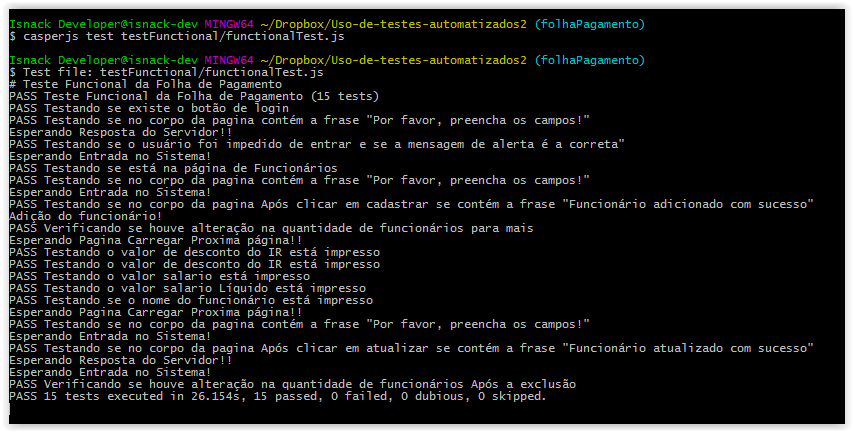
\includegraphics[width=13cm,height=13cm]{imagens/teste34.PNG}
   
     \textbf{Fonte: } Elaborado pelos autores.}
     \label{fig:Log dos testes executados com sucesso}
\end{figure}

\par A Figura 18 mostra o \textit{log} dos testes executados com sucesso, como pode-se reparar, no final é mostrado o tempo de execução de 26 segundos, mostrando assim, que os testes funcionais demoram um tempo maior para finalizar se comparados aos testes de unidade.

\par Na Figura 19 mostra-se um caso em que ocorreu um erro na execução do teste, ele mostra que o elemento especificado não foi encontrado, nesse caso há possibilidade do teste ter sido executado sem esperar a página carregar totalmente. Para fazer o teste passar é só colocar um tempo de esperar utilizando a função \texttt{wait}, como foi explicado durante os testes.


\begin{figure}[!htb]

     \caption[Teste mostrando erro]{Teste mostrando erro.
    \centering
      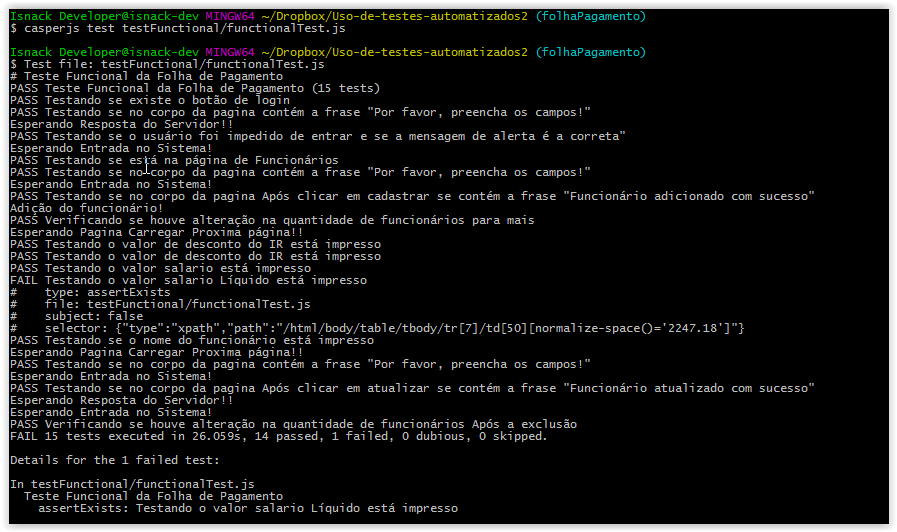
\includegraphics[width=13cm,height=13cm]{imagens/teste35.PNG}
   
     \textbf{Fonte: } Elaborado pelos autores.}
     \label{fig:Teste mostrando erro}
\end{figure}


\par O tempo de execução dos testes funcionais foi em média 26 segundos, se comparado com os testes de unidade e bem mais demorado.



\newpage
\section{TravisCI}

\par Para poder utilizar integração contínua, foi necessário configurar uma conta no \textit{TravisCI}.
 \par Primeiramente é feito a criação de um arquivo na raiz do projeto nomeado \texttt{travis.yml} esse arquivo será responsável pela configuração da \textit{build}. A Figura 20 é o exemplo de configuração.

\begin{figure}[!htb]

     \caption[Configuração inicial do TravisCI ]{Configuração inicial do TravisCI.
     \centering
      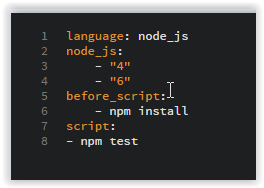
\includegraphics[width=12cm,height=6cm]{imagens/travis1.png}
   
     \textbf{Fonte: } Elaborado pelos autores.}
     \label{fig:configuração inicial do TravisCI}
\end{figure}


\begin{itemize}
 
 \item \textit{Language} é a definição da linguagem a ser usada na hora de criar a \textit{build} do projeto.
 
 \item \textit{Before script} é uma seção para especificar um comando antes de executar o \textit{script} principal, no projeto é executado para instalar todas as dependências que estão listadas no \texttt{package.json}.
 
 \item \textit{Script} é o lugar que será executado algum comando para execução dos testes e integração da solução. 
 
\end{itemize}

\par Após a criação do arquivo \texttt{travis.yml} é necessário dar permissão para o serviço \textit{TravisCI} acessar os repositórios da conta do \textit{GitHub}, e só utilizar a opção \textit{login} pelo \textit{GitHub} que automaticamente é pedido as permissões de acesso, então aceitá-las.
\par Com as permissões aceitas, é só adicionar o repositório desejado no \textit{TravisCI}, a Figura 20 demonstra essa ilustração.
 \newpage
\begin{figure}[!htb]
     \caption[Adicionar repositório no TravisCI ]{Adicionar repositório no TravisCI.
     \centering
     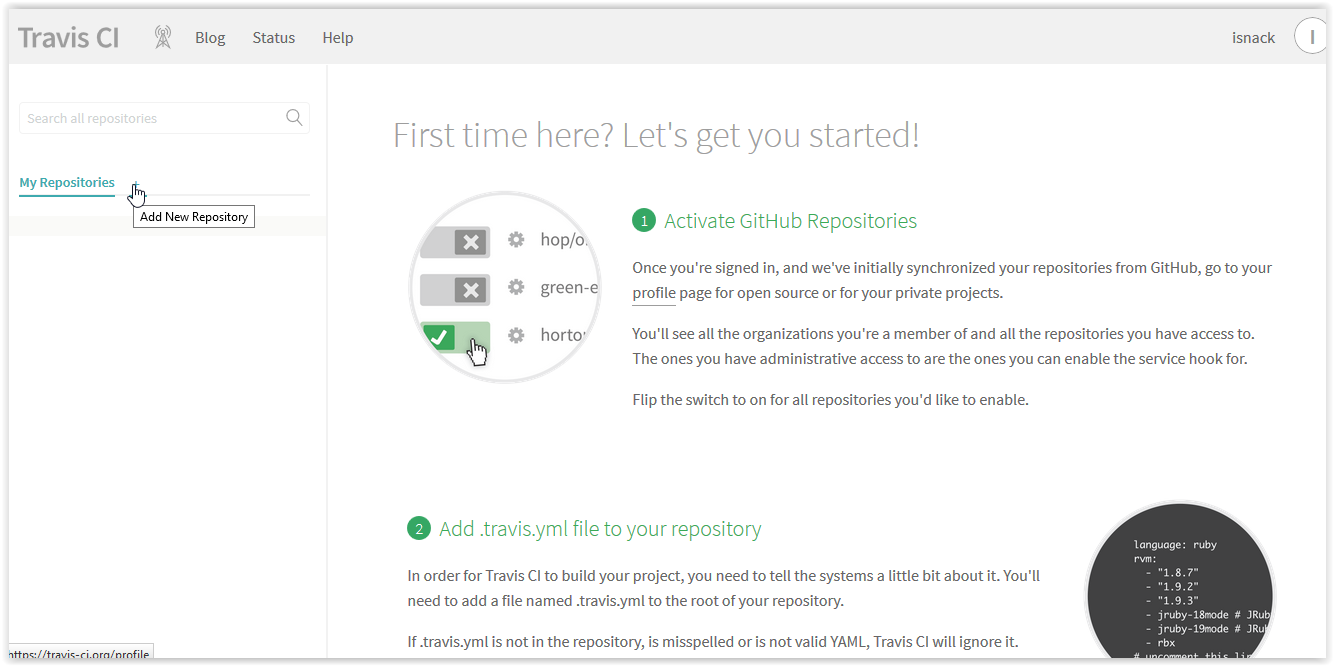
\includegraphics[width=12cm,height=6cm]{imagens/travis2.png}
    
     \textbf{Fonte: } Elaborado pelos autores.}
     \label{fig:adicionar repositório no TravisCI}
\end{figure}
 
 

\par Acessar \textit{Add New Repository} \footnote{Adicionar novo repositório}, caso seja a primeira vez que está acessando o \textit{TravisCI} é necessária uma sincronização com sua conta do \textit{GitHub}. A Figura 21 faz essa demonstração.

\begin{figure}[!htb]
    \caption[Sincronização do TravisCI com GitHub ]{Sincronização do TravisCI com GitHub.
     \centering
     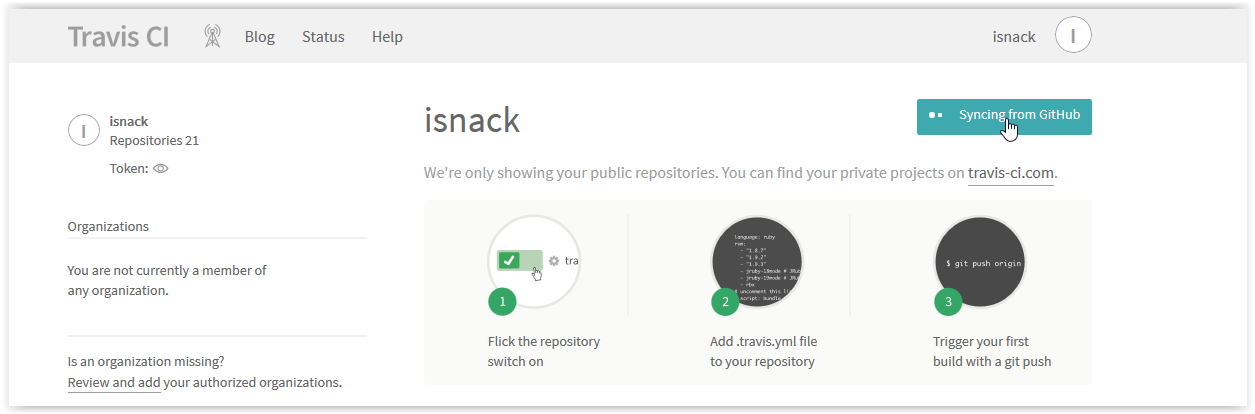
\includegraphics[width=12cm,height=6cm]{imagens/travis3.png}
     
     \textbf{Fonte: } Elaborado pelos autores.}
     \label{fig:sincronização do TravisCI com GitHub}
\end{figure}

\par Feita a sincronização da conta do \textit{GitHub} são listados todos os repositórios, selecionar o repositório em que serão feitos os testes, e feita a configuração, conforme mostra Figura 22.

\newpage
\begin{figure}[!htb]
    
    \caption[Repositório em que é feito a configuração do TravisCI  ]{Repositório em que é feito a configuração do TravisCI.
     \centering
     
\includegraphics[width=15cm,height=3cm]{imagens/travis4.png}
     
     \textbf{Fonte: } Elaborado pelos autores.}
     \label{fig:repositório em que é feito a configuração do TravisCI}
\end{figure}


\par Após a ação acima são apresentadas algumas configurações, conforme mostra Figura 24.

\begin{figure}[!htb]
    \caption[Configurações do TravisCI ]{Configurações do TravisCI.
     \centering
     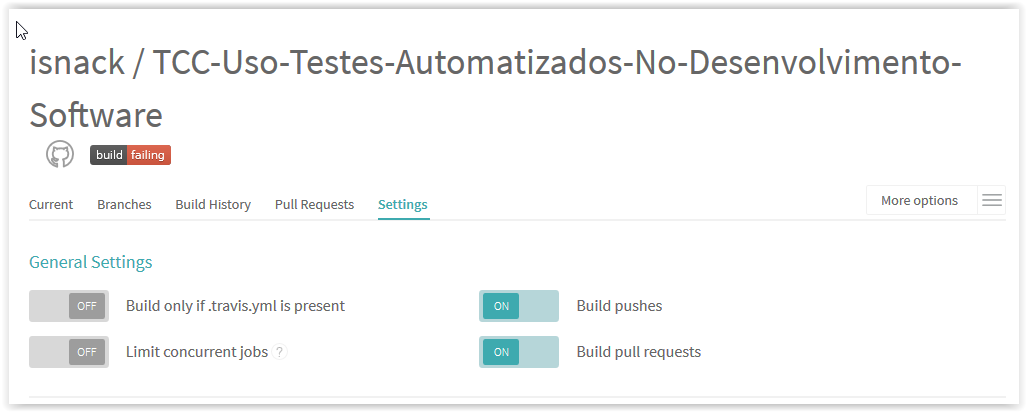
\includegraphics[width=12cm,height=6cm]{imagens/travis5.png}
     
     \textbf{Fonte: } Elaborado pelos autores.}
     \label{fig:configurações do TravisCI}
\end{figure}

\begin{itemize}
 
\item \textit{Build Pushes} é todo \textit{commit} ou alteração no código do repositório, o \textit{TravisCI} executará novamente a \textit{build}, executando todos os testes programados.

\item \textit{Build Only IF .travis.yml} o \textit{travisCI}, só irá executar uma integração se o arquivo de configuração estiver presente no repositório.
 
 \item \textit{Build pull requests}, é executado uma integração toda vez que tiver um \textit{pull request}
 
 \item \textit{Build History} é o local de armazenamento dos \textit{log} de todas as \textit{builds} executadas durante a criação do projeto.
 
\end{itemize}


\par Feito as configurações no repositório o \textit{Travis} está habilitado para testar a aplicação conforme mostra Figura 25.
\newpage
\begin{figure}[!htb]
    \caption[TravisCI está pronto para realização dos testes ]{TravisCI está pronto para realização dos testes.
     \centering
     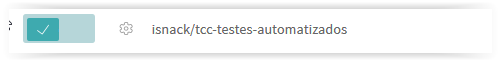
\includegraphics[width=15cm,height=3cm]{imagens/travis6.png}
      \textbf{Fonte: } Elaborado pelos autores.}
     \label{fig:TravisCI está pronto para realização dos testes}
\end{figure}

\par O primeiro \textit{commit} que foi feito no projeto, o \textit{travis} criará uma máquina virtual rodando o S.O \footnote{Sistema Operacional} Ubuntu, conforme mostra Figura 26.


\begin{figure}[!htb]
     \caption[TravisCI recebendo os commits ]{TravisCI recebendo os commits.
     \centering
     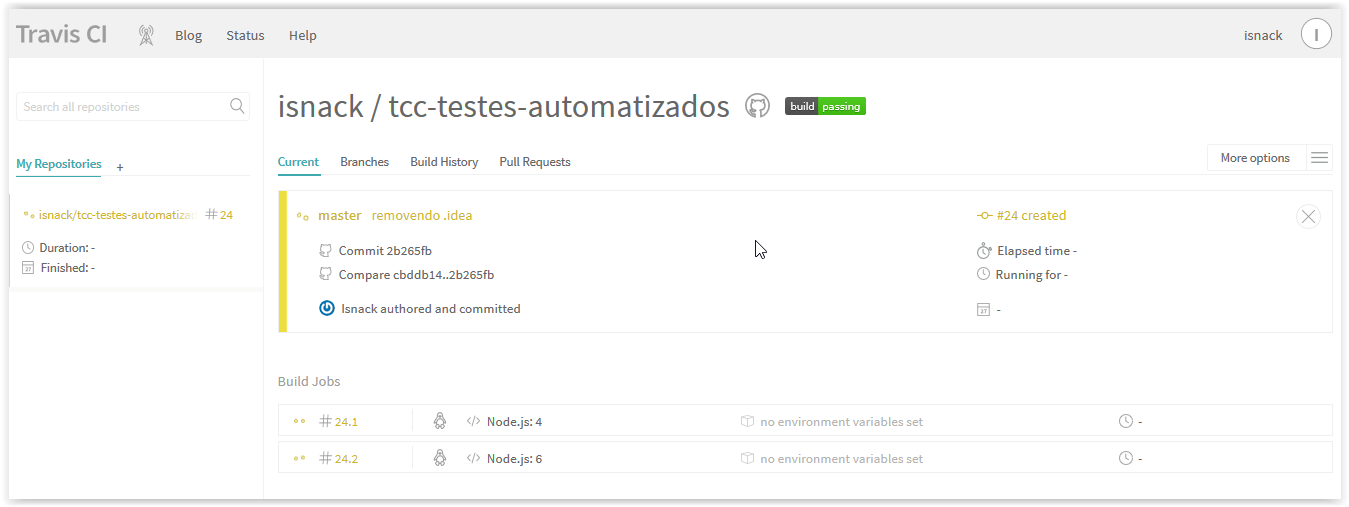
\includegraphics[width=15cm,height=9cm]{imagens/travis7.png}
      \textbf{Fonte: } Elaborado pelos autores.}
     \label{fig:travisCI recebendo os commits}
\end{figure}
 
 \par O projeto está sendo construído no repositório e sua cor fica em amarelo, para fazer essa referência, o \textit{Build Jobs} são as versões de linguagem, sinalizando que o seu projeto está sendo integrado e testado.

\par Na Figura 27 é mostrado o \textit{log} de inicialização do projeto, e pode se ver detalhes de como está sendo executado o projeto em si.
\newpage
\begin{figure}[!htb]
     \caption[Log de Inicialização ]{Log de Inicialização.
     
     \raggedleft
     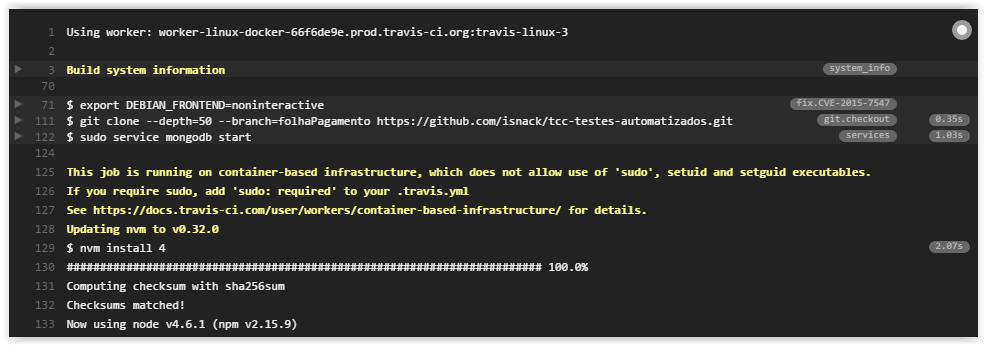
\includegraphics[scale=.60]{imagens/travis8.png}
     \centering
     \textbf{Fonte: } Elaborado pelos autores.}
     \label{fig:log de Inicialização}
\end{figure}


\par Após a execução do projeto, caso os testes falhem, o \textit{log} é responsável por mostrar para o desenvolvedor em qual linha ocorreu o erro, conforme mostra Figura 28.

\begin{figure}[!htb]
\centering
    \caption[Log mostrando o erro ]{Log mostrando o erro.
     
     
     \centering
     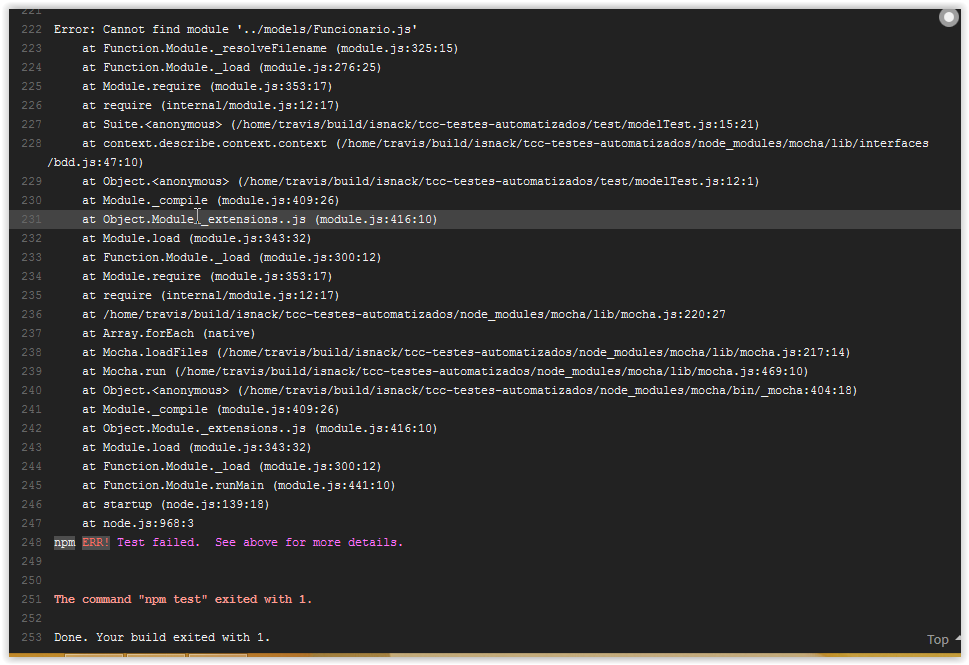
\includegraphics[width=15cm,height=9cm]{imagens/travis9.png}
     
     \centering
      \textbf{Fonte: } Elaborado pelos autores.}
     \label{fig:log mostrando o erro}
\end{figure}


\par Observando a Figura 28, o erro mostrado é o módulo do banco chamando o funcionário não encontrado, com esse \textit{feedback}, é necessário corrigir a chamada do módulo, para que seja executado com sucesso o teste. Caso os testes passem, é apresentado no painel a cor verde, indicando que os testes foram executados com sucesso. A Figura 29 mostra o \textit{log} no qual os testes passaram.

\newpage
\begin{figure}[!htb]
    \caption[Log com sucesso ]{Log com sucesso.
     
      \raggedleft
     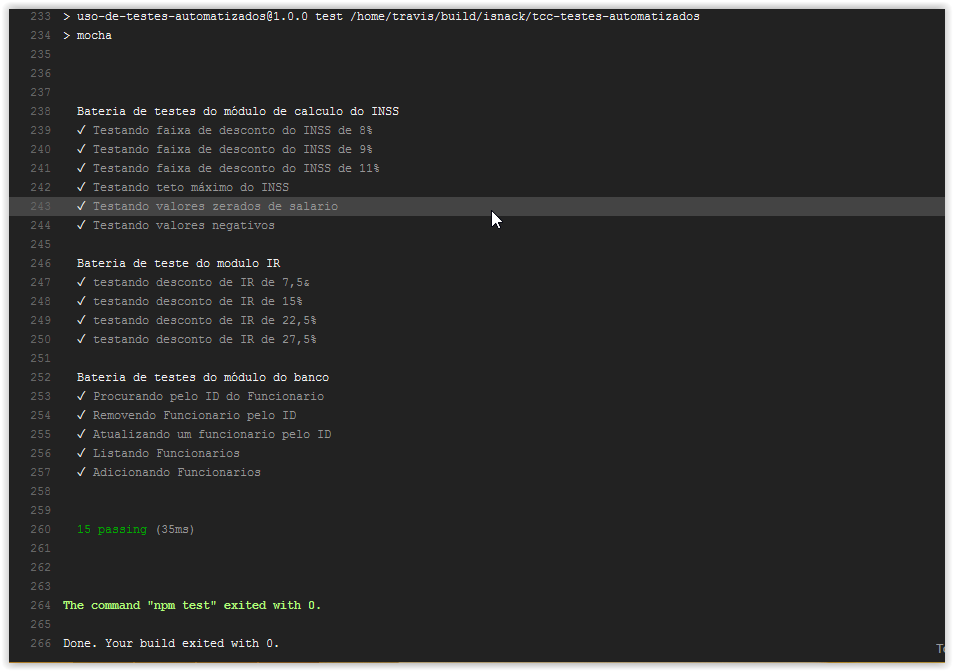
\includegraphics[width=15cm,height=9cm]{imagens/travis10.png}
     
     \centering
     \textbf{Fonte: } Elaborado pelos autores.}
     \label{fig:log com sucesso}
\end{figure}

\par O \textit{TravisCI} disponibiliza o histórico de tudo que foi feito no decorrer do projeto.
\par Essa funcionalidade ajuda muito o desenvolvedor a verificar como foi o andamento do projeto, e se houveram muitos erros que foram vistos e corrigidos no decorrer do desenvolvimento, a Figura 30 explica isso.

\begin{figure}[!htb]
    \caption[Históricos dos commits no TravisCI ]{Históricos dos commits no TravisCI.
     
     \raggedleft
     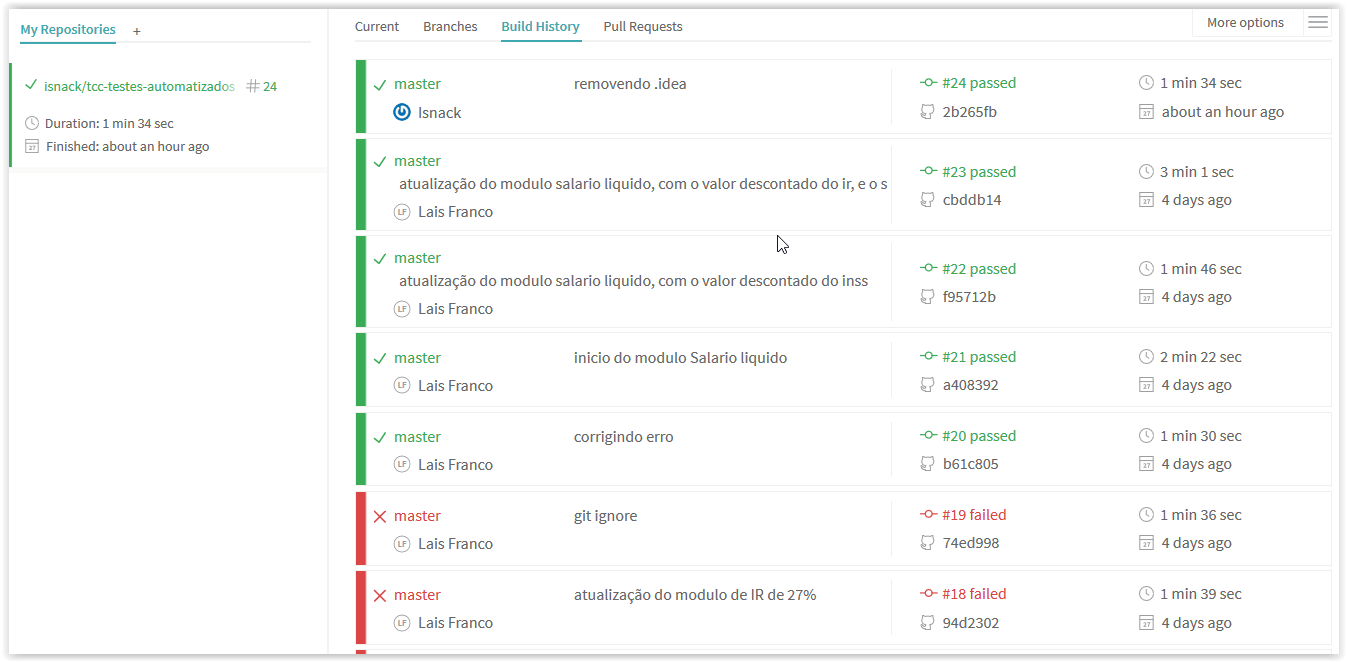
\includegraphics[width=15cm,height=9cm]{imagens/travis11.png}
     
     \centering
     \textbf{Fonte: } Elaborado pelos autores.}
     \label{fig:históricos dos commits no TravisCI}
\end{figure}

\newpage
\par Houve duas integrações que quebraram, e o autor corrigiu o erro, e novamente enviou com as alterações feitas, para que o projeto voltasse a funcionar normalmente. Durante esse processo todos os membros da equipe ficam a par do que está acontecendo, e se o responsável enviar uma \textit{build} quebrada outro membro da equipe pode resolver o problema.

\par O \textit{TravisCI} disponibiliza outro meio de ver os \textit{logs} de execução com ou sem sucesso.

\par Através do \textit{e-mail}, toda vez que um teste é executado os membros da equipe recebem um \textit{e-mail} mostrando se aquela versão está quebrada ou não, conforme mostra Figura 31.
 
\begin{figure}[!htb]
    \caption[E-mail que o TravisCI envia ]{E-mail que o TravisCI envia.
     \centering
     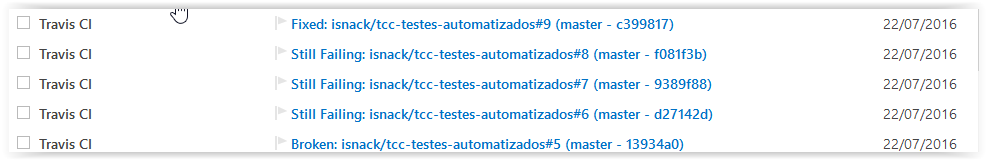
\includegraphics[width=14cm,height=3cm]{imagens/travis12.png}
     \textbf{Fonte: } Elaborado pelos autores.}
     \label{fig:e-mail que o TravisCI envia}
\end{figure}


\par Ao abrir a mensagem se vê mais detalhes e o link para o \textit{TravisCI}, e visualizar com detalhes o \textit{log} de inicialização, execução dos testes e o link para comparação do código antigo e o novo.



\par Outra funcionalidade é a integração contínua, quando se tem um \textit{pull request}, o \textit{TravisCI} executa a integração quando se tem uma nova contribuição no repositório. Conforme mostra a Figura 32, o \textit{TravisCI} executa a integração  quando se tem um \textit{pull request}.


\begin{figure}[!htb]
    \caption[Pull Request no TravisCi ]{Pull Request no TravisCi.
     \centering
     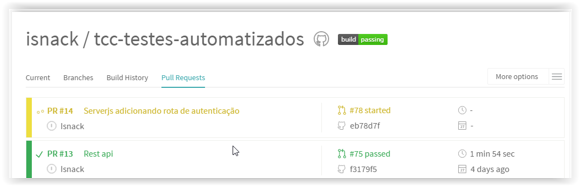
\includegraphics[width=12cm,height=6cm]{imagens/travis13.PNG}
     
     \textbf{Fonte: } Elaborado pelos autores.}
     \label{fig:Pull Request no TravisCi}
\end{figure}

\newpage
\par Assim o gerente ou o responsável pelo repositório não tem a necessidade de baixar a requisição e testar em uma máquina, o \textit{TravisCI} se encarrega dessa tarefa, desta forma, poupa-se tempo.

\par A Figura 33 apresenta um \textit{checklist} mostrando se a integração contínua está sem quebrar, desse jeito o botão de \textit{merge} no \textit{GitHub} fica verde, para efetuar o procedimento de junção do código.

\begin{figure}[!htb]
    \caption[Checklist ]{Checklist.
    
     \centering
     \includegraphics[width=12cm,height=6cm]{imagens/travis14.PNG}
     
     \textbf{Fonte: } Elaborado pelos autores.}
     \label{fig:Checklist}
\end{figure}


\par Caso contrário o \textit{checklist} fica com os itens em vermelho, indicando que teve falha na integração, conforme mostra a Figura 34.

\newpage
\begin{figure}[!htb]
    \caption[Checklist mostrando erro ]{Checklist mostrando erro.
    
     \centering
     \includegraphics[width=12cm,height=6cm]{imagens/travis15.PNG}
     
     \textbf{Fonte: } Elaborado pelos autores.}
     \label{fig:Checklist mostrando erro}
\end{figure}

\par Todos esses eventos são notificados por \textit{email}, assim toda equipe fica por dentro das integrações feitas no repositório.

\newpage
\section{Relatório de Cobertura}


\par Nessa seção é demonstrada a configuração do relatório de cobertura de testes para geração localmente e a utilização do serviço \texttt{coveralls.io}, esse relatório é necessário para obter a informação de como os testes criados no projeto estão cobrindo as unidades criadas.

\par Para isso primeiramente foi configurado o relatório localmente para esse propósito  é necessário instalar um pacote no NPM chamado \textit{istanbul}, com o seguinte comando \texttt{npm install istanbul –g}, esse pacote é rapidamente instalado.

\par Após esse procedimento, é necessário configurar na seção de \textit{scripts} do NPM, como mostra a Código 21.



\begin{lstlisting}[language=JavaScript, caption={[Configurar o relatório de cobertura com o NPM.]{Configurar o relatório de cobertura com o NPM.  \textbf{Fonte:} Elaborado pelos autores.}}]
"scripts":{
"test": "mocha",
"coveralls-local" : "istanbul cover ./node_modules/mocha/bin/_mocha"

},
\end{lstlisting}

\begin{comment}
\begin{figure}[!htb]
    \caption[Configurar o relatório de cobertura com o NPM  ]{Configurar o relatório de cobertura com o NPM.
    
     \centering
     \includegraphics[width=15cm,height=4cm]{imagens/relatorio.PNG}
     
     \textbf{Fonte: } Elaborado pelos autores.}
     \label{fig:Configurar o relatório de cobertura com o NPM}
\end{figure}
\end{comment}

\par Adicionando o comando coveralls-local: “istanbul cover ./node\_modules/mocha/Bin/\\\_mocha”, após realizar a configuração, foi executado comando npm run coveralls-local, deste modo foi criado uma pasta chamada \texttt{coverage} dentro do projeto e nela são criados arquivos em HTML os quais contém os relatórios de cobertura. A Figura 35 ilustra os arquivos contidos na pasta \texttt{coverage}.



\begin{figure}[!htb]
    \caption[Criado pasta coverage ]{Criado pasta coverage.
    
     \centering
     \includegraphics[width=15cm,height=4cm]{imagens/relatorio2.PNG}
     
     \textbf{Fonte: } Elaborado pelos autores.}
     \label{fig: Criado pasta coverage}
\end{figure}


\newpage

\par Ao abrir a pasta \texttt{lcov-report}, contém um arquivo chamado \texttt{index.html} e ao executar o mesmo, será apresentado o relatório de cobertura, como pode ser observado na Figura 36 o relatório separa por pasta.

\begin{figure}[!htb]
    \caption[lcov-report ]{ lcov-report.
    
     \centering
     \includegraphics[width=15cm,height=4cm]{imagens/relatorio3.PNG}
     
     \textbf{Fonte: } Elaborado pelos autores.}
     \label{fig:lcov-report}
\end{figure}

\par Dentro da pasta \texttt{services} contém todas unidades ou arquivos que contém lógica e nas quais os testes foram executados, o relatório exibe algumas informações como:

\begin{itemize}
 \item \textit{Statements}: Porcentagem de cobertura dos testes, ou seja, quantos por cento do código testado está sendo coberto pelo teste;
 \item \textit{Branches}: Cobertura nos \textit{Branches};
 \item \textit{Functions}: Cobertura nas funções;
 \item \textit{Lines}: Cobertura de linhas no código.
 
\end{itemize}

\begin{figure}[!htb]
    \caption[Relatório de Cobertura ]{Relatório de Cobertura.
    
     \centering
     \includegraphics[width=15cm,height=4cm]{imagens/relatorio4.PNG}
     
     \textbf{Fonte: } Elaborado pelos autores.}
     \label{fig:Relatório de Cobertura}
\end{figure}

\par A Figura 37 mostra que o código está com mais de 85\% coberto pelos testes, além do arquivo que está com o menor índice de cobertura, que nesse caso é de mais de 52\%, enquanto os outros arquivos estão com 100\% de cobertura.

\par Abrindo uma unidade com 100\% de cobertura e outra com 52\%, observa-se algumas informações.

\newpage
\begin{figure}[!htb]
    \caption[Relatório de Cobertura no qual  está 52\% coberto ]{Relatório de Cobertura no qual  está 52\% coberto.
    
     \centering
     \includegraphics[width=15cm,height=15cm]{imagens/relatorio5.PNG}
     
     \textbf{Fonte: } Elaborado pelos autores.}
     \label{fig:Relatório de Cobertura no qual não está 52\% coberto}
\end{figure}

\par A Figura 38 mostra quais as linhas estão necessitando que faça-se um teste, e essas linhas ficam destacadas em vermelho para facilitar a sua visualização.
\par A Figura 39 mostra um código que está com 100\% de cobertura, por isso fica tudo verde.

\newpage

\begin{figure}[!htb]
    \caption[Relatório de Cobertura no qual  está 100\% coberto ]{Relatório de Cobertura no qual  está 100\% coberto.
    
     \centering
     \includegraphics[width=12cm,height=10cm]{imagens/relatorio6.PNG}
     
     \textbf{Fonte: } Elaborado pelos autores.}
     \label{fig:Relatório de Cobertura no qual não está 100\% coberto}
\end{figure}

\par O relatório de cobertura demonstra que o projeto necessita de mais testes, e assim,  auxiliando no desenvolvimento dos testes no sistema que está sendo desenvolvido.

\par Feito a configuração da cobertura de testes localmente, também foi configurado \textit{online} utilizando o site \url{http://www.coveralls.io}.

\par O procedimento é a criação de uma conta no site citado acima, pode se utilizar a integração com \textit{GitHub} para criação da conta, sendo possível fazer a sincronização dos repositórios do \textit{GitHub}.

\begin{figure}[!htb]
    \caption[Sincronizando Github com o coveralls ]{Sincronizando Github com o coveralls.
    
     \centering
     \includegraphics[width=8cm,height=5cm]{imagens/relatorio7.PNG}
     
     \textbf{Fonte: } Elaborado pelos autores.}
     \label{fig:Sincronizando Github com o coveralls}
\end{figure}

\newpage

\par Feito a criação da conta no site, no menu do lado esquerdo  tem a opção \textit{add repositoy} (conforme mostra Figura 40), após esse procedimento  são listados todos os repositórios do \textit{GitHub}, depois é só habilitar o repositório da aplicação. Conforme mostra a Figura 41.

\begin{figure}[!htb]
    \caption[Listas de repositórios no GitHub ]{Listas de repositórios no GitHub.
    
     \centering
     \includegraphics[width=15cm,height=4cm]{imagens/relatorio9.PNG}
     
     \textbf{Fonte: } Elaborado pelos autores.}
     \label{fig:Listas de repositórios no GitHub}
\end{figure}

\begin{figure}[!htb]
    \caption[O setup do relatório de cobertura utilizando o TravisCI ]{O setup do relatório de cobertura utilizando o TravisCI.
    
     \centering
     \includegraphics[width=12cm,height=8cm]{imagens/relatorio8.PNG}
     
     \textbf{Fonte: } Elaborado pelos autores.}
     \label{fig:O setup do relatório de cobertura utilizando o TravisCI}
\end{figure}

\par Após a habilitação do repositório, a Figura 42 mostra como realizar o \textit{setup} do relatório de cobertura utilizado o serviço de integração contínua (\textit{TravisCI}). Com esses dados foi necessário criar o arquivo \texttt{.coveralls.yml}, nesse arquivo contém o parâmetro \texttt{repo\_token} que é um numero de identificação do repositório no site do \textit{coverlls}.
\par A Figura 43 demonstra a criação do arquivo \texttt{.coveralls.yml}, na pasta raiz do projeto e na Figura 44 o conteúdo do arquivo. 

\newpage

\begin{figure}[!htb]
    \caption[Criação do .coveralls.yml ]{Criação do .coveralls.yml.
    
     \centering
     \includegraphics[scale=1]{imagens/relatorio10.PNG}
     
     \textbf{Fonte: } Elaborado pelos autores.}
     \label{fig:Criação do .coveralls.yml}
\end{figure}

\begin{figure}[!htb]
    \caption[Rebo Token ]{Repo Token.
    
     \centering
     \includegraphics[scale=1]{imagens/relatorio11.PNG}
     
     \textbf{Fonte: } Elaborado pelos autores.}
     \label{fig:Rebo Token}
\end{figure}

\par Após esses procedimentos, foi necessária a instalação de um pacote, o \textit{coveralls} utilizando o npm , o comando \texttt{npm install coveralls  -- save} e depois a configuração do \textit{script} dentro do arquivo \texttt{package.json}.




\begin{lstlisting}[language=JavaScript, caption={[Configuração do script dentro do package.json.]{Configuração do script dentro do package.json.  \textbf{Fonte:} Elaborado pelos autores.}}]
"scripts": {
  "test": "mocha",
  "coveralls-local": "istanbul cover ./node_modules/mocha/bin/_mocha",
  "coveralls": "istanbul cover ./node_modules/mocha/bin/_mocha --report lcovonlu -- -R spec && cat ./coverage/lcov.info | ./node_modules/coveralls/bin/coveralls.js && rm -rd ./coverage"
 } 


\end{lstlisting}

\begin{comment}


\begin{figure}[!htb]
    \caption[Configuração do script dentro do package.json ]{Configuração do script dentro do package.json.
    
     \centering
     \includegraphics[width=16cm,height=4cm]{imagens/relatorio12.PNG}
     
     \textbf{Fonte: } Elaborado pelos autores.}
     \label{fig:Configuração do script dentro do package.json}
\end{figure}
\end{comment}

\par O Código 22 mostra a criação do \textit{script} chamado \textit{coveralls}, no qual o comando utilizado é “istanbul cover ./node\_modules/mocha/bin/\_mocha --report lcovonly -- -R spec \&\& cat ./coverage/lcov.info |   ./node\_modules/coveralls/bin/coveralls.js && rm -rf ./coverage”.


\par Esse \textit{script} roda o teste, cria o relatório de cobertura localmente e lê o arquivo \texttt{lcov.info}, no qual contém as informações de cobertura do teste e envia essas informações para o arquivo \texttt{coveralls.js}, que por sua vez, envia todas essas informações para o site do \textit{coveralls.io}.

\par Foi necessário adicionar mais uma linha de comando no arquivo \texttt{.travis.yml} que é o responsável pela integração com \textit{TravisCI}, foi adicionada a instalação do \textit{istanbul} no setor  \textit{before\_script}, no setor \textit{after\_script} e adicionado o \textit{script}  \texttt{npm run coveralls}, que será executado logo após o \textit{script} principal de integração. Conforme mostra Figura 45.

\begin{figure}[!htb]
    \caption[Adicionando linhas de comando no .travis.yml ]{Adicionando linhas de comando no .travis.yml.
    
     \centering
     \includegraphics[width=16cm,height=9cm]{imagens/relatorio13.PNG}
     
     \textbf{Fonte: } Elaborado pelos autores.}
     \label{fig:Adicionando linhas de comando no .travis.yml}
\end{figure}

\par Após realizar as configurações, deve-se fazer algum \textit{commit} ou \textit{pull request}, o relatório é gerado após a integração feita pelo \textit{TravisCI}. A Figura 46 demonstra um relatório gerado pelo site \url{www.coveralls.io}.


\begin{figure}[!htb]
    \caption[Relatório gerado pelo coveralls.io ]{Relatório gerado pelo coveralls.io.
    
     \centering
     \includegraphics[width=15cm,height=8cm]{imagens/relatorio14.PNG}
     
     \textbf{Fonte: } Elaborado pelos autores.}
     \label{fig:Relatório gerado pelo coveralls.io}
\end{figure}

\newpage
\par O relatório demonstra as mesmas informações do que é gerado localmente como: cobertura do arquivo, linhas, quais dessas linhas são relevantes e as linhas de maior relevância estão cobertas.

\par Um exemplo interessante ao se criar um \textit{pull request} é a integração do \textit{coveralls.io} com \textit{GitHub}, o site notifica a porcentagem de cobertura e se a cobertura se manteve ou se caiu comparando com o código atual. A Figura 47 faz essa demonstração.

\begin{figure}[!htb]
    \caption[Notificação de porcentagem de cobertura ]{Notificação de porcentagem de cobertura.
    
     \centering
     \includegraphics[width=15cm,height=9cm]{imagens/relatorio15.PNG}
     
     \textbf{Fonte: } Elaborado pelos autores.}
     \label{fig:Notificação de porcentagem de cobertura}
\end{figure}


\par Nesse caso, a cobertura dos testes era de 100\% e teve uma redução de mais de 14\%, essa informação é de grande relevância, pois a partir dela decide-se quando aceitar o \textit{pull request}  e se o responsável pelo projeto requer uma porcentagem específica de cobertura dos testes ou não.

\par No \textit{coveralls.io} é possível criar uma configuração, que caso o \textit{pull request} tiver uma cobertura menor que 90\% seja considerado como falha, ou então se a cobertura cair uma porcentagem específica também é considerado como falha. Para esse propósito basta acessar o repositório que está com relatório de cobertura e clicar no link \textit{Settings} como mostra a Figura 48.

\newpage
\begin{figure}[!htb]
    \caption[Configuração do coveralls.io ]{Configuração do coveralls.io.
    
     \centering
     \includegraphics[width=12cm,height=7cm]{imagens/relatorio16.PNG}
     
     \textbf{Fonte: } Elaborado pelos autores.}
     \label{fig:Configuração do coveralls.io}
\end{figure}

\par A opção \textit{Coverage threshold for failure} é opção de alerta quando a cobertura cair abaixo de 90\% como ilustra a Figura 48. E a opção \textit{Coverage decrease threshold for failure} alerta quando a cobertura cair uma porcentagem que pode ser especificada, Ex: mais de 15\% será emitido um alerta.

\par A Figura 49 mostra um \textit{branch} que não está de acordo com as regras especificadas, ficando assim marcado com um “x” em vermelho indicando que não está de acordo.

\begin{figure}[!htb]
    \caption[Branch que não está de acordo com as regras especificadas ]{Branch que não está de acordo com as regras especificadas.
    
     \centering
     \includegraphics[scale=0.60]{imagens/relatorio17.PNG}
     
     \textbf{Fonte: } Elaborado pelos autores.}
     \label{fig:Branch que não está de acordo com as regras especificadas}
\end{figure}
\begin{comment}


\newpage
\section{Participantes}

\par Isnack e Laís foram os responsáveis pelo planejamento, execução e testes do \textit{software} e também análise e desenvolvimento da pesquisa e suas conclusões.

\par Isnack Souza Novais, Técnico em informática formado pelo INPETTECC, possui experiência em desenvolvimento com linguagem de programação ".NET" e manipulação de banco de dados SQL SERVER, cursando o 8º período do Curso de Sistemas de Informação
da Universidade do Vale do Sapucaí.

\par Laís Vidal de Oliveira, cursando 8º período do curso de Sistemas de Informação da Universidade do Vale do Sapucaí e fazendo curso de Testes Automatizados e C\#. 

\par Ednardo David Segura – Pós-graduado em Engenharia Web pela Universidade Federal de Itajubá – UNIFEI (2008). Possui graduação em Ciência da Computação pelo Centro de Ensino Superior em Gestão, Tecnologia e Educação – FAI (2006). Atualmente é Especialista em Sistemas Sênior do Inatel Competence Center e Professor em cursos de Pós-Graduação no INATEL e da graduação na Univás. Possui experiência em desenvolvimento de software nas linguagens JavaScript (client/server), Java SE/EE, PHP, Groovy, para a plataforma web atuando principalmente nos seguintes temas: Telecomunicações, IPTV/OTT e Cloud Computing. Possui bons conhecimentos em programação orientada a objetos, programação funcional e desenvolvimento orientado a testes.

\end{comment}


\clearpage
\newpage

\begin{comment}

\section{Cronograma}

\par Abaixo descrito no cronograma as ações a serem seguidas no projeto, desde a definição até a conclusão.

\begin{figure}[!htb]
     \centering
 \includegraphics[width=17cm,height=17cm]{imagens/cronograma6.png}
     \caption[Cronograma do desenvolvimento do projeto]{Cronograma do desenvolvimento do projeto.
     \textbf{Fonte: } Elaborado pelos autores.}
     \label{fig:cronograma}
\end{figure}

\clearpage
\newpage

\section{Orçamento}
\par Abaixo o orçamento com as despesas detalhadas previstas para a realização do projeto.

\begin{figure}[!htb]
     \centering
     \includegraphics[width=17cm,height=17cm]{imagens/orcamento.png}
     \caption[Orçamento previsto do projeto]{Orçamento previsto do projeto.
     \textbf{Fonte: } Elaborado pelos autores.}
     \label{fig:orcamento}
\end{figure}


\end{comment}










\begin{comment}
Exemplo de código Java:

\begin{lstlisting} [style=custom_Java,caption={[Métodos da classe \texttt{FilmeBean}]{Métodos da classe \texttt{FilmeBean}. \textbf{Fonte:} Elaborado pelos autores.}}, label=fig:metodosclassebean] 	
	public FilmeBean(){  
       //...
   	}	
   	
	public void saveMovie(){
		setListActorSelected();		
		if(this.movieDAO.saveMovieGraph(this.movieTo)){
			FacesContext.getCurrentInstance().addMessage(null, 
			   new FacesMessage("Filme cadastrado com sucesso!")); 
		}else{
			//...
		}		
		this.limpaCampos();
	}
\end{lstlisting}

\par Agora será mostrado o exemplo do uso de fluxo de eventos apresentado no Quadro~\ref{quad:fluxo_evento_cadastro_filme}.

\begin{quadro}[h!]
  \begin{fluxoDeEventos}
  \addTitle{Cadastrar filme}
  \addrow{Ator principal}{Administrador}
  %\addrow{Ator secundário}{Sistema de cartão}
  \addrow{Pré-requisitos}{Estar logado no sistema}

  \startBasicFlow{Ator} {Sistema}
  \addItemOne{Seleciona menu cadastro}
  \addItemOne{Clica na opção cadastrar filme}
  \addItemTwo{Abre interface de cadastro de filme}
  \addItemOne{Preenche formulário}
  \addItemOne{Clica no botão salvar}
  \addItemTwo{Salva e informa sucesso no cadastro}

  \startAlternativeFlow{Fluxo alternativo 1}
  \addItemOne{No item 5, formulário não preenchido}
  \addItemTwo{Exibe mensagem de necessidade de preenchimento de formulário}

  \startAlternativeFlow{Fluxo alternativo 2}
  \addItemOne{No item 6, inserido filme já cadastrado}
  \addItemTwo{Informa mensagem de filme já cadastrado}
\end{fluxoDeEventos}

  \caption[Fluxo de eventos para cadastro de filme]
           {Fluxo de eventos para cadastro de filme. \textbf{Fonte:} Elaborado pelos autores}
  \label{quad:fluxo_evento_cadastro_filme}
\end{quadro}

\par Outro exemplo é ilustrado na Figura~\ref{fig:bluesky}. Neste caso um código XML foi embutido dentro de um ambiente de figura, para que este código seja incluído no índice de figuras adequadamente.
 
\begin{figure}[ht!]
  \begin{lstlisting} [style=custom_XML]
	...
	<context-param>
		<param-name>primefaces.THEME<\param-name>
		<param-value>bluesky<\param-value>
	<\context-param>
	...
  \end{lstlisting}
 
  \caption[Incluindo o tema \textit{BlueSky} ao contexto do projeto]
          {Incluíndo o tema \textit{BlueSky} ao contexto do projeto. \textbf{Fonte:} Elaborado pelos autores.}
  \label{fig:bluesky}
\end{figure}
\end{comment}
\chapter{ DISCUSSÃO DE RESULTADOS} 


\par Neste capítulo são apresentados e discutidos os resultados obtidos na pesquisa realizada sobre o uso de testes automatizados no desenvolvimento de \textit{software} com o objetivo de destacar suas características, pontos principais e benefícios dessa abordagem.

\par Conforme citado em capítulos anteriores, o cenário utilizado para a demonstração de resultados foi um sistema web para a simulação de resultados de uma folha de pagamento. Através do uso do desenvolvimento orientado a testes (TDD), pôde-se perceber que há um grande benefício em se tratando de receber respostas de regressão, informações de problemas e falhas nas funcionalidades desenvolvidas para o sistema. 

\par Caso uma outra metodologia de desenvolvimento fosse adotada para o sistema que não o TDD, problemas seriam detectados tardiamente, visto que não haveria uma abordagem focada em testes tal como o TDD prega.





% \par Por isso o desenvolvimento orientado a teste (TDD) é muito mais rápido e eficaz.


\begin{figure}[!htb]
\centering
    \caption[TDD e Desenvolvimento Tradicional  ]{TDD e Desenvolvimento Tradicional.
     
     \raggedleft
     \includegraphics[scale=.35]{imagens/tdd.png}
     \centering
     \textbf{Fonte: } Elaborado pelos autores.}
     \label{fig:TDD e Desenvolvimento Tradicional}
\end{figure}


\par Vê-se, na Figura 50, como a metodologia TDD faz uso de testes: a cada porção de funcionalidade desenvolvida, há um ou mais testes automatizados desenvolvidos especialmente para garantir que aquele trecho irá funcionar conforme esperado e que todos os possíveis erros serão tratados. Com isso, pode-se prevenir erros futuros que já foram encontrados no momento do desenvolvimento do sistema. 

\par Já no segundo exemplo, vê-se que as funcionalidades são criadas e só então os testes são criados para estas. Muitas vezes, cenários deixam de ser cobertos pelos testes nessa metodologia, gerando uma porcentagem maior de falhas nos resultados finais.

\par Utilizando o desenvolvimento orientado a teste, obtém-se uma resposta rápida sobre se o módulo está funcionando corretamente, e assim, prevenir erros à frente. No exemplo da Figura 51, é demonstrado que os testes foram executados com sucesso, conforme o esperado.



\begin{figure}[!htb]
    \caption[Testes INSS Passando  ]{Testes INSS Passando.
     \centering
     
     \includegraphics[width=12cm,height=8cm]{imagens/teste9.png}
     
     \textbf{Fonte: } Elaborado pelos autores.}
     \label{fig:testes INSS passando}
\end{figure}


\par A Figura 51 demonstra o uso de testes para cobrir várias possibilidades de uso do método o qual está sendo testado. No caso acima exemplificado, foi escolhida uma determinada porcentagem, a qual seria enviada para a funcionalidade que calcula o desconto do INSS (sobre o salário bruto do funcionário) para que esta retornasse um determinado resultado. Foi utilizado o \textit{framework} \textit{chai} e \textit{mocha} para facilitar a criação dos testes.




\par Este trabalho utilizou \textit{frameworks} para facilitar as realizações dos testes, criando vários cenários ou baterias de testes, sendo que, nesse cenário se específica o módulo que será testado. O Código 15 demonstra uma bateria de testes realizados neste trabalho

\clearpage
\newpage

    
\begin{comment}
    
\begin{figure}[!htb]
   \caption[Criação de todos os testes INSS ]{Criação de todos os teste INSS.
     \centering
     
     \includegraphics[width=12cm,height=6cm]{imagens/teste7.png}
     
     \textbf{Fonte: } Elaborado pelos autores.}
     \label{fig:todos teste inss}
\end{figure}

\end{comment}



\begin{lstlisting}[language=JavaScript, caption={[Criação de todos os testes INSS.]{Criação de todos os testes INSS.  \textbf{Fonte:} Elaborado pelos autores.}}]
var expect = require('chai').expect;
var inssService = require('../app/services/INSSService');

describe('Bateria de testes do módulo de calculo do INSS',function(){
    
    it('Testando faixa de desconto do INSS de 8%',function(){
        expect(inssService.calculate(1000)).to.equal(80);
    });
    it('Testando faixa de desconto do INSS de 9%',function(){
        expect(inssService.calculate(1700)).to.equal(153);
    });
    it('Testando faixa de desconto do INSS de 11%',function(){
        expect(inssService.calculate(2700)).to.equal(297);
    });
    it('Testando teto máximo do INSS',function(){
        expect(inssService.calculate(5980.96)).to.equal(570.88);
    });
    it('Testando valores zerados de salario',function(){
        expect(inssService.calculate(0)).to.equal(0);
    });
    it('Testando valores negativos',function(){
        expect(inssService.calculate(-1569)).to.equal(0);
    });
});

\end{lstlisting}



\par O Código 15, demonstra como os testes foram criados: um teste foi criado para cada possibilidade de desconto do INSS para um determinado salário bruto enviado para a funcionalidade. Os testes da Figura 51 finalizaram com sucesso, pois obedeciam o critério definido nos testes.

\par Comparado com os testes manuais os testes funcionais demonstraram um bom resultado na produtividade dos testes devido a sua automação para testar toda a funcionalidade da aplicação. Porém os testes funcionais tem um custo elevado devido a dificuldade do seu desenvolvimento em comparação ao desenvolvimento dos testes de unidade e integração.
 
 \par Um dos principais benefícios alcançados por esta pesquisa, foi a utilização da integração contínua (\textit{TravisCI}), sendo que, se a \textit{build} quebrar ou não, o \textit{TravisCI} encaminha um \textit{e-mail} avisando sobre a ocorrência. 
 
\par Uma grande vantagem de receber as notificações por \textit{e-mail}, é que hoje em dia todas as pessoas tem seu \textit{e-mail} sincronizado com seu \textit{smartphone}. Isso facilita a vida do desenvolvedor, pois assim que ocorre um evento, ele é notificado. Conforme mostra a Figura 52.
 
 
\begin{figure}[!htb]
    \caption[E-mail TravisCI envia ]{E-mail TravisCI envia.
     \centering
     \includegraphics[width=14cm,height=3cm]{imagens/travis12.png}
     \textbf{Fonte: } Elaborado pelos autores.}
     \label{fig:e-mail TravisCI envia}
\end{figure}


\par Conforme a Figura 53, esse é o exemplo do \textit{e-mail} aberto logo após ser recebido e aberto na caixa de entrada. Sendo possível verificar o que está acontecendo no repositório.

\begin{figure}[!htb]
\centering
    \caption[E-mail aberto  ]{E-mail aberto.
    
     
     
     \includegraphics[scale=.75]{imagens/travis30.PNG}
     
     \textbf{Fonte: } Elaborado pelos autores.}
     \label{fig:e-mail aberto}
\end{figure}



\par Além de notificações via \textit{e-mail}, o \textit{TravisCI} também disponibiliza a integração na ocasião da integração de um \textit{pull request}; ou seja, qualquer contribuição é previamente testada pelo serviço antes que uma junção (\textit{merge}) seja efetivada com sucesso, a fim de evitar qualquer erro e/ou problema com o código atual. 

\par Se houver um problema com a integração, a ferramenta envia uma mensagem de \textit{e-mail} ao responsável para que o mesmo esteja ciente dos problemas que o código presente no \textit{pull request} podem potencialmente causar.

\par Há um \textit{check-list} com o resultado da integração: quais arquivos têm problema, quais foram responsáveis pela falha de determinados testes, dentre outros. Isso gera uma segurança e tranquilidade maior por parte dos desenvolvedores, pois podem previamente detectar problemas e erros antes que novas atualizações sejam atreladas ao produto atual.


\begin{figure}[!htb]
    \caption[Pull Request dando erro ]{Pull Request dando erro.
    
     \centering
     \includegraphics[width=12cm,height=6cm]{imagens/travis15.PNG}
     
     \textbf{Fonte: } Elaborado pelos autores.}
     \label{fig:Pull Request dando erro}
\end{figure}


\par A Figura 54 demonstrada é resultado de uma integração que apresenta problemas. Quando o \textit{pull request} foi feito, todos os interessados puderam realizar comentários e analisar as mudanças antes da mesma ser adicionada ao código de produção, a fim de garantir que potenciais problemas sejam evitados antes mesmo que as alterações sejam adicionadas ao produto.

\par Outro benefício foi a utilização do relatório de cobertura, o qual verifica a porcentagem de trechos de código que são verificados pelos testes e quais linhas de códigos ainda não são. Para os trechos que não estão sendo verificados, deve-se adicionar um grupo de testes para melhorar os índices de sucesso do relatório de cobertura.

\par Na Figura 55, as linhas em vermelho representam o número de linhas que faltam ser verificadas por testes automatizados e que necessitam de uma atenção especial.

\newpage

\begin{figure}[!htb]
    \caption[Relatório de Cobertura no qual tem partes que não estão cobertas ]{Relatório de Cobertura no qual tem partes que não estão cobertas.
    
     \centering
     \includegraphics[width=15cm,height=15cm]{imagens/relatorio5.PNG}
     
     \textbf{Fonte: } Elaborado pelos autores.}
     \label{fig:Relatório de Cobertura no qual tem partes que não estão cobertas}
\end{figure}


\par Observa-se na Figura 55 que, após a análise de um desenvolvedor experiente, há a necessidade de uma melhoria no projeto, implementando e aprimorando testes nas unidades que ainda não estão cobertas e/ou não são verificadas. Com isso, o índice de cobertura do  projeto aumenta, melhorando os resultados posteriores ao buscar relatórios de testes automatizados.

\par Outra vantagem que o relatório de cobertura oferece é a integração com o \textit{coveralls.io} (ferramenta que proporciona o uso do relatório de cobertura online), o qual disponibiliza funcionalidades para gerenciar a porcentagem mínima aceitável de cobertura de testes. Caso esse índice não seja atingido, o código a ser integrado é considerado como falha. %Conforme mostra Figura 56.

\begin{figure}[!htb]
    \caption[Pull request dando erro no relatório de cobertura]{Pull request dando erro no relatório de cobertura.
    
     \centering
     \includegraphics[scale=1.0]{imagens/discussao2.PNG}
     
     \textbf{Fonte: } Elaborado pelos autores.}
     \label{fig:Pull request dando erro no relatório de cobertura}
\end{figure}


\newpage
\par Como se pode observar na Figura 56, o \textit{coveralls.io} faz integração com o \textit{GitHub} e o \textit{TravisCI}. Toda vez que um \textit{pull request} é enviado, a ferramenta faz a análise do trecho de código enviado. Após a análise, um ícone em vermelho representa a porcentagem de código o qual não está propriamente verificado/coberto através de testes automatizados (o responsável pelo repositório ainda poderá realizar a mesclagem com o código principal; porém, um \textit{e-mail} será enviado aos interessados alertando a porcentagem de cobertura do código para aquele \textit{pull request} enviado).

\par Conclui-se que o uso de ferramentas de testes automatizados é benéfico aos desenvolvedores de \textit{software}, auxiliando-os a entregar sistemas com o menor índice possível de falhas e erros (\textit{bugs}), os quais são detectados com antecedência através do uso dessas ferramentas. A satisfação do cliente se torna maior ao usar um \textit{software} com o mínimo de erros possíveis.




\begin{comment}
    

\par A figura acima mostra que foram testadas várias possibilidades de testes, sendo que em cada possibilidade executada especificou-se uma determinada porcentagem, que se refere ao desconto do INSS sobre o salário bruto do funcionário.


\par A figura acima demonstra uma maneira simplificada do que foi falado acima, sendo que o vermelho representa os testes e o azul o desenvolvimento do sistema.
\par O objetivo da pesquisa foi demonstrar através da criação de uma folha de pagamento web, a utilização dos testes automatizados.   


\par No processo de desenvolvimento orientado a testes (TDD), percebe-se que ao criar os testes e executá-los, há uma resposta rápida se o método está funcionando corretamente.


\par Está resposta rápida não é obtida com sucesso quando usado os testes manuais ou desenvolvimento tradicional, pois nesse processo, se desenvolve boa parte do sistema antes de aplicar os testes e a verificação se está funcionando corretamente ou não.


\par Se usar os testes manuais ou o desenvolvimento tradicional, que nada mais é do que desenvolver boa parte do sistema para depois aplicar os testes e assim verificar se está tudo funcionando corretamente, as repostas obtidas iram demorar um pouco mais, do que usar o desenvolvimento orientado a testes.
\par Entre os principais benefícios alcançados por esta pesquisa, pode-se afirmar que o \textit{pull-request} desempenho um grande 



\par Neste capítulo tem por finalidade descrever os resultados obtidos nesta pesquisa através de uma explicação teórico-prática. 

\par O presente trabalho teve por objetivos desenvolver testes automatizados, mostrando assim que quando mais teste são feitos, menor e o índice do \textit(software) apresentar falhas, sendo possível ter um índice de cobertura do sistema maior.

\par o objetivo da pesquisa foi demonstrar como o uso de testes automatizados detém a melhorar significativamente o desenvolvimento de uma folha de pagamento web.

 \end{comment}








\chapter{CONSIDERAÇÕES FINAIS} 
\begin{comment}
\par A conclusão deste trabalho é \ldots

\par Assim conclui-se que \ldots
\end{comment}


\par Com a realização desta pesquisa, foi criado um sistema de folha de pagamento \textit{web} utilizando testes automatizados, foram descritos o funcionamento dos testes, a preparação de um ambiente de desenvolvimento e a demonstração do funcionamento dos testes automatizados, e com isso, se cria um \textit{software} com um índice menor de falhas.

\par Foi utilizado em conjunto com os testes automatizados, a integração contínua, que visa a cada nova melhoria no código estar verificando se isso não vai ocasionar nenhuma falha ou até mesmo quebrar a \textit{build}, com isso o desenvolvedor garante cada vez mais entregar no final um \textit{software} de qualidade e com menos \textit{bugs}.

\par E também, em conjunto aos testes foi utilizado o relatório de cobertura cujo seu principal objetivo é alertar os desenvolvedores sobre a porcentagem que o código está coberto, como é possível verificar qual parte do código necessita de mais testes, para aumentar esse índice de cobertura.

\par O principal objetivo desse trabalho foi demonstrar que a utilização de testes no desenvolvimento de software contribui para o aumento da qualidade da aplicação a ser desenvolvida, prevenindo erros que possam ocorrer em uma aplicação.

\par Por fim, pode-se afirmar que o presente trabalho realizou seus  objetivos,os quais eram: desenvolver uma folha de pagamento \textit{web}, na qual iria proporcionar a realização dos testes automatizados que foram propostos por este trabalho, proporcionando um maior conhecimento na utilização de testes automatizados de \textit{softwares} e seus mais variados tipos, para começar a desenvolver utilizando a prática de desenvolvimento de software TDD (desenvolvimento orientado a teste) que requer um esforço maior, porque é uma prática diferente do que a maioria dos desenvolvedores estão acostumados, em meio essa dificuldade, percebeu-se que com a utilização dos testes nessa prática de desenvolvimento, consegue-se evitar erros no final do projeto, pois foram realizados testes em todo o processo de desenvolvimento do sistema.

\par Ainda, esta pesquisa foi de grande relevância aos participantes do projeto, pois contribui para uma ampla visão sobre os benefícios de se utilizar testes automatizados em todo o desenvolvimento do \textit{software} e um conhecimento vasto nas tecnologias utilizadas.

\par Como futuros trabalhos sugerimos a utilização do BDD (Behavior Driven Development) e das ferramentas para análise na qualidade do código, pois este apresenta uma abordagem diferenciada, interessante e com mais vantagens ainda em sua utilização.




\postextual %Início dos Elementos Pós-Textuais

%\citeoption{abnt-etal-cite=2}
%\cite{ABNT-final}
%\input{biblio}

\bibliography{biblio}{}
 \addcontentsline{toc}{chapter}{\protect\numberline{}REFERÊNCIAS}
%\addcontentsline{toc}{chapter}{REFERÊNCIAS} % adiciona o título no sumário






\begin{apendicesenv}

%\apendicesname{APÊNDICES}
% Imprime uma página indicando o início dos apêndices
\partapendices*

\addcontentsline{toc}{chapter}{APÊNDICES}












\chapter*{Pesquisa sobre a Importância de se utilizar teste automatizados}
\label{apendice:1}

\par Nesta apêndice são mostradas as perguntas que foram feitas através do google \textit{forms}, para obter dados relevantes sobre, se os desenvolvedores utilizam testes automatizados no processo de desenvolvimento do \textit{software}.
\par Na Figura 57 estão todas as perguntas que foram feitas.

\begin{figure}[!htb]
    \caption[Perguntas sobre a importância de se utilizar teste automatizados ]{Perguntas sobre a importância de se utilizar teste automatizados.
    
     \centering
     \includegraphics[width=12cm,height=25cm]{imagens/perg4.PNG}
     
     \textbf{Fonte: } Elaborado pelos autores.}
     \label{fig:Perguntas sobre a importância de se utilizar teste automatizados}
\end{figure}

\begin{comment}

Na Figura 55, 56 e 57 é ilustrada a primeira pergunta da pesquisa.

\begin{figure}[!htb]
    \caption[Perguntas sobre a importância de se utilizar teste automatizados ]{Perguntas sobre a importância de se utilizar teste automatizados.
    
     \centering
     \includegraphics[width=18cm,height=8cm]{imagens/perg1.PNG}
     
     \textbf{Fonte: } Elaborado pelos autores.}
     \label{fig:Perguntas sobre a importância de se utilizar teste automatizados}
\end{figure}

\begin{figure}[!htb]
    \caption[Perguntas sobre a importância de se utilizar teste automatizados ]{Perguntas sobre a importância de se utilizar teste automatizados.
    
     \centering
     \includegraphics[width=18cm,height=8cm]{imagens/perg2.PNG}
     
     \textbf{Fonte: } Elaborado pelos autores.}
     \label{fig:Perguntas sobre a importância de se utilizar teste automatizados}
\end{figure}

\begin{figure}[!htb]
    \caption[Perguntas sobre a importância de se utilizar teste automatizados ]{Perguntas sobre a importância de se utilizar teste automatizados.
    
     \centering
     \includegraphics[width=18cm,height=20cm]{imagens/perg3.PNG}
     
     \textbf{Fonte: } Elaborado pelos autores.}
     \label{fig:Perguntas sobre a importância de se utilizar teste automatizados}
\end{figure}

\end{comment}



\begin{comment}

\captionsetup[figure]{list=no}
\begin{figure}[h!]
 \centerline{\includegraphics[scale=0.5]{./imagens/perg1.PNG}}
 \caption[Outra imagem.]
           {Outra imagem. \textbf{Fonte:} Elaborado pelos autores}
  \label{fig:ap1:identificador}
\end{figure}

\par Após a seleção do tipo de projeto \ldots
 ~\ref{apendice:1}.
\end{comment}
\begin{comment}



\chapter*{Título do Apêndice 2}

\section*{Primeira seção do apêndice 2}

\par Neste apêndice é mostrado \ldots de acordo com a Figura~\ref{fig:ap2:identificador} é ilustrada a primeira tela deste processo.
\captionsetup[figure]{list=no}
\begin{figure}[h!]
 \centerline{\includegraphics[scale=0.3]{./imagens/apendice_img1.png}}
 \caption[Outra imagem ainda.]
           {Outra imagem ainda. \textbf{Fonte:} Elaborado pelos autores}
  \label{fig:ap2:identificador}
\end{figure}

\section*{Segunda seção do apêndice 2}

\begin{comment}


\par Continuando \ldots na figura Figura~\ref{fig:xml_exemplo} é mostrado um exemplo de XML.

\begin{figure}[h!]
\begin{lstlisting}[style=custom_XML]
<project>
...
 <dependencies>
  ...
  <dependency>
   <groupId>org.neo4j</groupId>
   <artifactId>neo4j</artifactId>
   <version>1.9.4</version>
  </dependency>
  ...
 </dependencies>
 ...
</project>
\end{lstlisting}  
 \caption[Exemplo de código XML.]
           {Exemplo de código XML. \textbf{Fonte:} Elaborado pelos autores}
  \label{fig:xml_exemplo}
\end{figure}


\end{comment}

\end{apendicesenv}






%\anexoname{ANEXOS}
%\begin{anexosenv}
%\partanexos
%

\begin{comment}



\chapter*{}

\begin{figure}[!htb]
     \centering
     \includegraphics[width=17cm,height=20cm]{imagens/revisao.png}
     
    
 
\end{figure}

\end{comment}
%\end{anexosenv}

\addcontentsline{toc}{chapter}{ANEXOS}



\begin{comment}



\chapter*{}

\begin{figure}[!htb]
     \centering
     \includegraphics[width=17cm,height=20cm]{imagens/revisao.png}
     
    
 
\end{figure}

\end{comment}



\end{document}
